% \section*{JAVA}
\section{Introduction}
As reported in the state of the art, Java is one of the most popular programming languages adopted by practitioners.In fact, in 2022, Java will be second only to Python, according to PYPY~\footnote{\url{https://pypl.github.io/PYPL.html}}.
Furthermore, if we take into consideration legacy applications, Java becomes the most used programming language.According to the TIOBE index, Java was the most frequently used language from 2002 until 2017, and it remained in the top 5 after that~\footnote{\url{https://www.tiobe.com/tiobe-index/}}.
In addition to its popularity, Java exhibits an interesting behavior when it comes to energy consumption and performance, Java applications can be at the same time one of the most energy-efficient or hungry solutions.
As we have seen in the previous chapter, an inappropriate combination of parameters can drive Java applications from the top language to the bottom just by setting the wrong parameters.
in this chapter, we want to dig deeper into this aspect of Java and study its runtime.
This chapter thus focuses on the impact of the runtime of Java applications on energy consumption.

\subsection{Characteristics of JVM}
\begin{figure}%[ht]
    \centering
    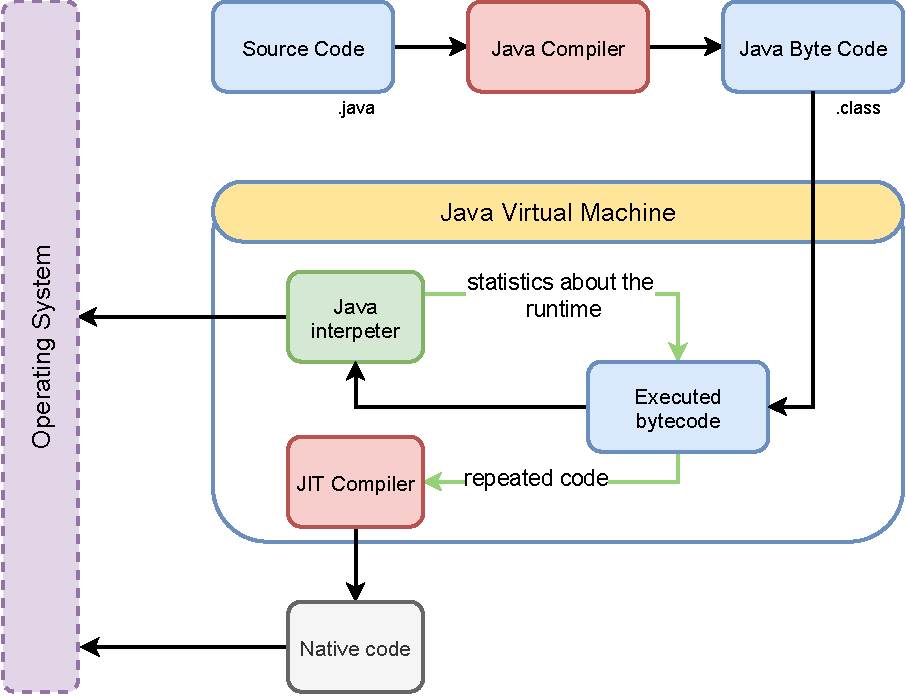
\includegraphics[width=\linewidth]{imgs/Jvm_architecture}
    \caption{JVM architecture}
    \label{fig:JVM_architecture}
\end{figure}

Java's portability is a core design goal, which means that Java applications will work exactly the same on any operating system and on any hardware.As we see in figure~\ref{fig:JVM_architecture}, Instead of machine code, this is accomplished by compiling Java language code to an intermediate representation known as Java bytecode. Java bytecode instructions are similar to machine code, but they are executed by a JVM rather than directly on the machine. As a result, Java programs will run slower and consume more memory than C++ programs. However, Just-in-Time (JIT) compilation, which is built into the JVM, improves performance by converting bytecode to machine code at runtime. Furthermore, an automatic garbage collector (GC) is used by Java to manage memory throughout the object lifecycle and to recover memory when objects are no longer in use.

\subsection{Research questions}
In this section, we will investigate the following research questions:
\begin{compactenum}[\indent\bf RQ\,1:]
    \item \emph{What is the impact of existing JVM distributions on the energy consumption of Java-based software services?}
    \item \emph{What are the relevant JVM settings that can reduce the energy consumption of a given software service?}
\end{compactenum}

To answer those research questions, we conduct an empirical study to highlight the impact of this runtime.

\section{Experimental Protocol}\label{sec:javaprotocol}
To investigate the effect that can have the JVM distribution choice and/or parameters on software energy consumption, we conducted a wide set of experiments on a cluster of machines and used several established Java benchmarks and JVM configurations.

\subsection{Measurement Contexts}

\noindent\textbf{Software Settings.}
For the sake of reproducibility, each experiment runs within a Docker container based on \textsf{SDKMAN}\footnote{\url{https://sdkman.io}} image and Alpine docker.\footnote{\url{https://github.com/alpinelinux/docker-alpine}}

\vspace{6pt}
\noindent\textbf{Hardware Settings.}
To report on reproducible measurements, we used the cluster \textsf{Dahu} from the G5K platform~\cite{grid5000} for most of our experiments.
This cluster is composed of $32$ identical compute nodes, which are equipped with $2$ Intel Xeon\,Gold\,6130 and 192\,GB of RAM.
Our experimental protocol enforces that the software under test is the only process executed on the node configured with a very minimal Linux Debian\,9 (4.9.0 kernel version).
The minimal OS configuration ensures that only mandatory services and daemons are kept active to conduct robust experiments and reduce the factors that can affect the energy consumption measurements during our experiments~\cite{opaper}.

\vspace{6pt}
\noindent\textbf{Java Virtual Machines Candidates.}
We considered a set of $52$ JVM distributions taken from $8$ different providers/packagers mostly obtained from \textsf{SDKMAN}, as listed in \Cref{tab:JVM}.
Depending on providers, either all the versions, majors, or LTS are made available by \textsf{SDKMAN}.

\begin{table}
    \centering
    \caption{List of selected JVM distributions.}
    \label{tab:JVM}
    \resizebox{\linewidth}{!}{
        \begin{tabular}{|c|c|c|l|}
            \hline
            \textbf{Distribution} & \textbf{Provider}       & \textbf{Support} & \textbf{Selected versions}                                               \\
            \hline
            \hline
            \textsc{HotSpot}      & \textbf{Adopt\,OpenJDK} & {\sc All}        & 8.0.275, 11.0.9, 12.0.2, 13.0.2, 14.0.2, 15.0.1                          \\
            \hline
            \textsc{HotSpot}      & \textbf{Oracle}         & {\sc All}        & 8.0.265, 9.0.4, 10.0.2, 11.0.2, 12.0.2, 13.0.2, 14.0.2, 15.0.1, 16.ea.24 \\
            \hline
            \textsc{Zulu}         & \textbf{Azul\,Systems}  & {\sc All}        & 8.0.272, 9.0.7, 10.0.2, 11.0.9, 12.0.2, 13.0.5, 14.0.2, 15.0.1           \\
            \hline
            \textsc{SapMachine}   & \textbf{SAP}            & {\sc All}        & 11.0.9, 12.0.2, 13.0.2, 14.0.2, 15.0.1                                   \\
            \hline
            \textsc{Librca}       & \textbf{BellSoft}       & {\sc All}        & 8.0.275, 11.0.9, 12.0.2, 13.0.2, 14.0.2, 15.0.1                          \\
            \hline
            \textsc{Corretto}     & \textbf{Amazon}         & {\sc Mjr}        & 8.0.275, 11.0.9, 15.0.1                                                  \\
            \hline
            \textsc{HotSpot}      & \textbf{Trava\,OpenJDK} & LTS              & 8.0.232, 11.0.9                                                          \\
            \hline
            \textsc{Dragonwell}   & \textbf{Alibaba}        & LTS              & 8.0.272, 11.0.8                                                          \\
            \hline
            \textsc{OpenJ9}       & \textbf{Eclipse}        & {\sc All}        & 8.0.275, 11.0.9, 12.0.2, 13.0.2, 14.0.2, 15.0.1                          \\
            \hline
            \textsc{GraalVM}      & \textbf{Oracle}         & LTS              & 19.3.4.r8, 19.3.4.r11, 20.2.0.r8, 20.2.0.r11                             \\
            \hline
            \textsc{Mandrel}      & \textbf{Redhat}         & LTS              & 20.2.0.0                                                                 \\
            \hline
        \end{tabular}
    }
\end{table}

\subsection{Workload}
We ran our experiments across $12$ Java benchmarks we picked from \textsf{OpenBenchmarking.org}.\footnote{\url{https://openbenchmarking.org}}
This includes $5$ acknowledged benchmarks from the \textsc{Dacapo} benchmark suite v.\,9.12~\cite{DaCapo:paper}, namely \textsf{Avrora}, \textsf{H2}, \textsf{Lusearch}, \textsf{Sunflow} and \textsf{PMD}, that have been widely used in previous studies and proven to be accurate for memory management and computer architecture~\cite{DBLP:conf/wosp/LengauerBMW17,DBLP:conf/oopsla/KaliberaMJV12}.
It consists of open-source and real-world applications with non-trivial memory loads.
% 
Then, we also considered $7$ additional benchmarks from the \textsc{Renaissance} benchmark suite~\cite{renaissance,DBLP:conf/pldi/ProkopecRLD0SBZ19}, namely \textsf{ALS}, \textsf{Dotty}, \textsf{Fj-kmeans}, \textsf{Neo4j}, \textsf{Philosophers}, \textsf{Reaction} and \textsf{Scrabble}, which offer a diversified set of benchmarks aimed at testing JIT, GC, profilers, analyzers, and other tools.
The benchmarks we picked from both suites exercise a broad range of programming paradigms, including concurrent, parallel, functional, and object-oriented programming.
\Cref{tab:benchmarks} summarizes the selected benchmarks with a short description. Meanwhile, Figure~\ref{fig:jvm-benchmarks-classification} highlights the scope of each benchmark from the test suite.


\begin{table*}
    \centering
    \caption{List of selected open-source Java benchmarks taken from \textsc{Dacapo} and \textsc{Renaissance}.}
    \label{tab:benchmarks}
    \resizebox{\linewidth}{!}{
        \begin{tabular}{|p{0.1\linewidth}|p{0.6\linewidth}|p{0.3\linewidth}|}
            \hline
            \textbf{Benchmark}    & {\bf Description}                                                                                                    & \textbf{Focus}                             \\
            \hline
            \hline
            \textsf{ALS}          & Factorize a matrix using the alternating least square algorithm on spark                                             & Data-parallel, compute-bound               \\
            \hline
            \textsf{Avrora}       & Simulates and analyses for AVR microcontrollers                                                                      & Fine-grained multi-threading, events queue \\
            \hline
            \textsf{Dotty}        & Uses the dotty Scala compiler to compile a Scala codebase                                                            & Data structure, synchronization            \\
            \hline
            \textsf{Fj-Kmeans}    & Runs K-means algorithm using a fork-join framework                                                                   & Concurrent data structure, task parallel   \\
            \hline
            \textsf{H2}           & Simulates an SQL database by executing a TPC-C like benchmark written by Apache                                      & Query processing, transactions             \\
            \hline
            \textsf{Lusearch}     & Searches keywords over a corpus of data comprising the works of Shakespeare and the King James bible                 & Externally multi-threaded                  \\
            \hline
            \textsf{Neo4j}        & Runs analytical queries and transactions on the Neo4j database                                                       & Query Processing, Transactions             \\
            \hline
            \textsf{Philosophers} & Solves dining philosophers problem                                                                                   & Atomic, guarded blocks                     \\
            \hline
            \textsf{PMD}          & Analyzes a list of Java classes for a range of source code problems                                                  & Internally multi-threaded                  \\
            \hline
            \textsf{Reactors}     & Runs a set of message-passing workloads based on the reactors framework                                              & Message-passing, critical-sections         \\
            \hline
            \textsf{Scrabble}     & Solves a scrabble puzzle using Java streams                                                                          & Data-parallel, memory-bound                \\
            \hline
            \textsf{Sunflow}      & Renders a classic Cornell box; a simple scene comprising two teapots and two glass spheres within an illuminated box & Compute-bound                              \\
            \hline
        \end{tabular}
    }
\end{table*}


\begin{figure*}%[ht]
    \centering
    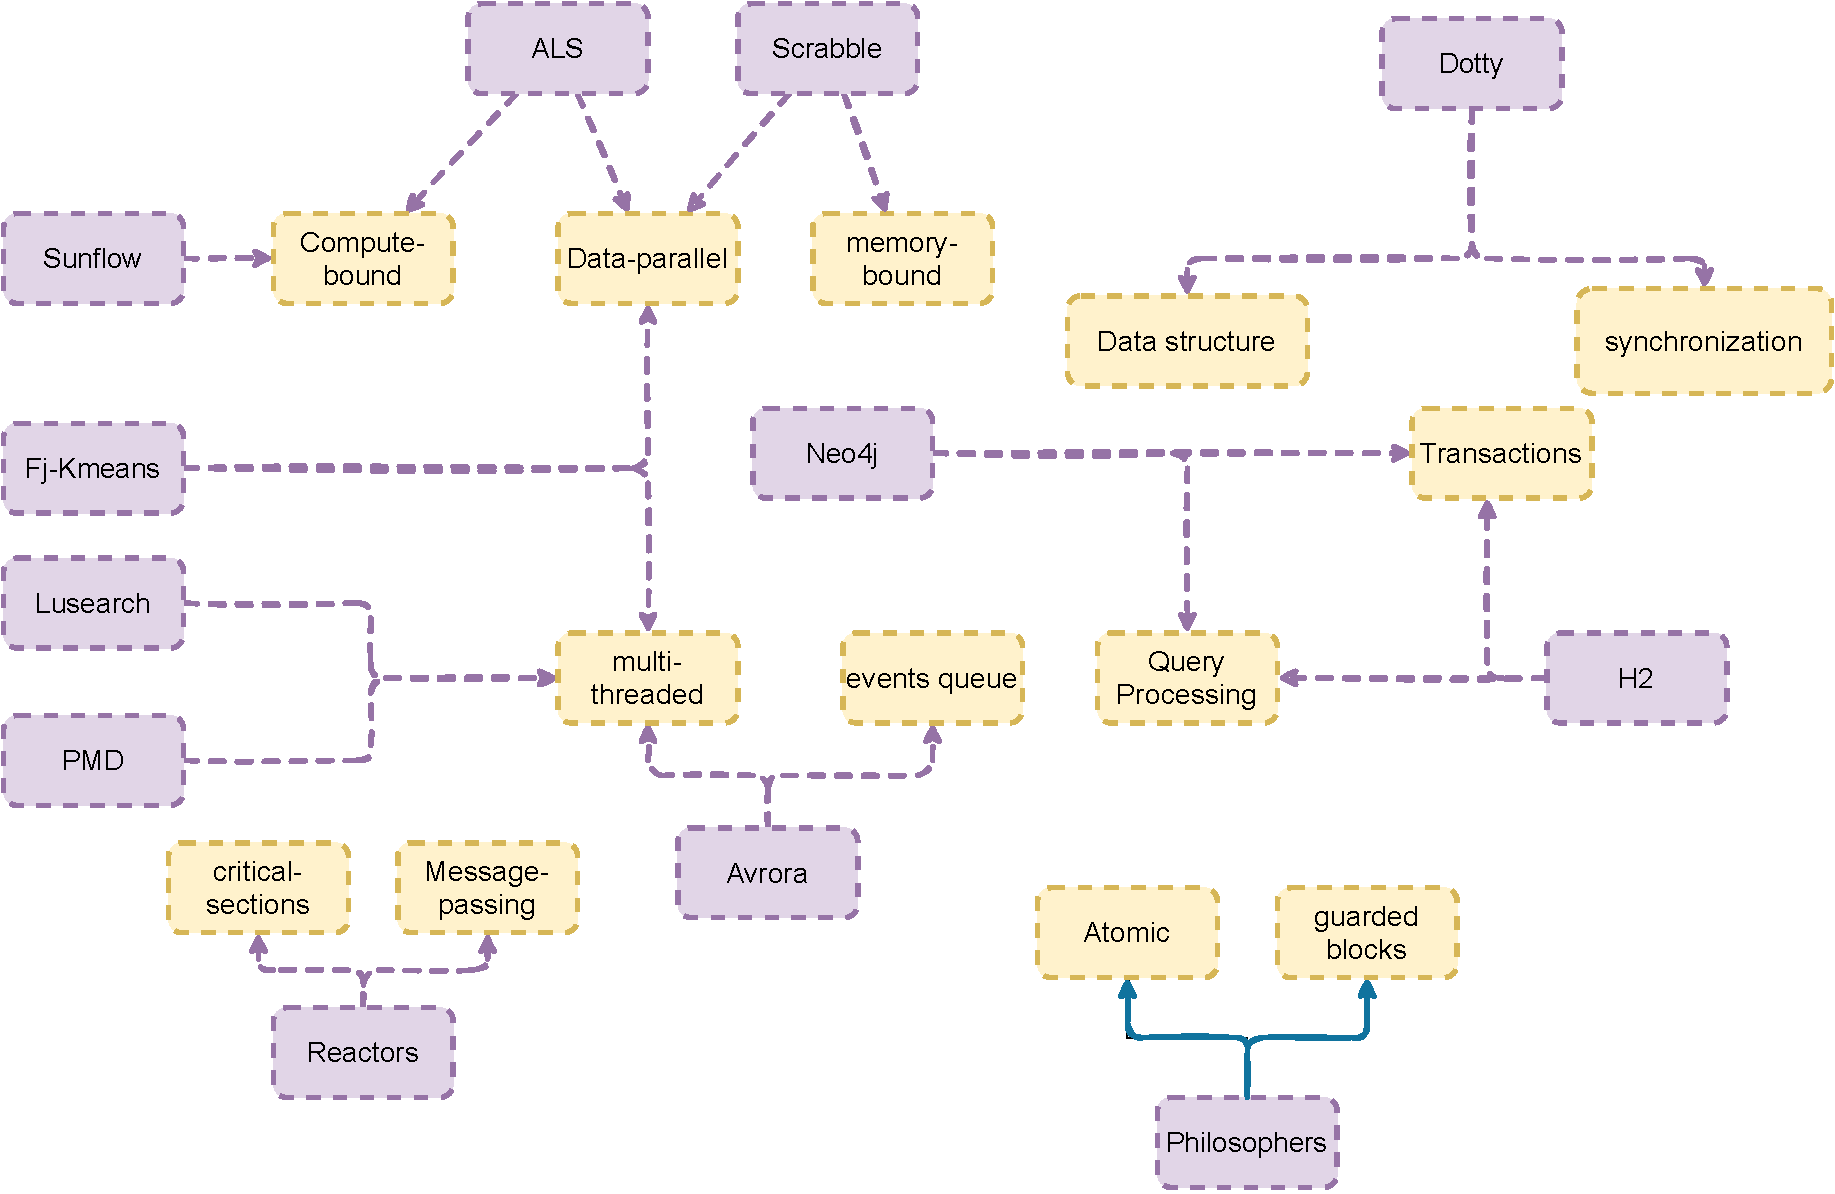
\includegraphics[width=\linewidth]{imgs/jvm_benchmarks}
    \caption{Target scope of \textsc{Dacapo} and \textsc{Renaissance} benchmarks.}
    \label{fig:jvm-benchmarks-classification}
\end{figure*}

\subsection{Metrics and Measurement}
Since the goal of this study is the green aspect of JVM, our key metric will be the energy consumed by job completed for each JVM configuration.
In addition to the energy consumption, we collected additional metrics to explain the reasons behind the behavior of each experiment.
Those additional metrics are:
\begin{itemize}
    \item execution time,
    \item number of threads.
\end{itemize}

% Our protocol allow the user to record extra metrics, such as the energy consumption of the memory, the CPU usage, etc.
% However, we focus only the the previous metrics.

\noindent\textbf{Energy Measurements.}
We used Intel\,RAPL as a physical power~meter to analyze the energy consumption of the CPU package and the DRAM.
RAPL is one of the most accurate tools to report on the global energy consumption of a processor~\cite{Khan:2018:RAE:3199681.3177754,10.1145/2989081.2989088}.
We note that, due to CPU energy consumption variations issues~\cite{opaper}, we used the same node for all our experiments.
% In other words, we used the same node to ran all the JVM from the different providers and with numerous configurations for each single benchmark application.
Moreover, we tried to be very careful, while running our experiments, not to fall in the most common benchmarking "crimes"~\cite{DBLP:journals/corr/abs-1801-02381}.
Every single experiment, therefore, reports on energy metrics obtained from at least $20$ executions of $50$ iterations per benchmark.
All of our experiments are available for use/reproducibility from our anonymous repository.\footnote{\url{https://anonymous.4open.science/r/jvm-comparaison-213E/Readme.md}}


\noindent\textbf{Number of threads.}
To collect the number of active threads used by the experiment, we use the command \texttt{top} and record at fixed intervals.

\subsection{Extension}
We also added an extension to the protocol to allow the user to run the same experiment with different configurations.
The package is available in the GitHub repository.\footnote{\url{https://github.com/chakib-belgaid/jvm-comparaison}}
To add extra \textbf{jvm candidates} for the benchmark applications, we added a new configuration file \texttt{jvm.sh} in the root directory of the repository, where we put the name and the version of the jvm to be used.
For the \textbf{input workload},the benchmarks should be provided in the \texttt{benchmarks} directory.
As for extra \textbf{metrics}, one can create a new script file that monitors the experiment and record the metrics.
We provide some examples, such as \texttt{recordpower.sh} to measure the instantaneous power and \texttt{recordthreads.sh} to measure the number of active threads during the experiment.

For faster experiments, we propose \textsc{Jreferral}\footnote{\url{https://github.com/chakib-belgaid/jreferral}}, an open source tool that automatically compares the JVM energy consumption and recommends the most energy-efficient configuration for a given Java application.
We further discuss this tool in Section~\ref{section:SummaryofContributions}.


\section{Experiments \& Results}\label{sec:exp}
\subsection{Energy Impact of JVM Distributions}
\noindent\textbf{Job-oriented applications.}
To answer our first research question, we executed $62,400$ experiments by combining the $52$ JVM distributions with the $12$ Java benchmarks, thus reasoning on $100$ energy samples acquired for each of these combinations.
\Cref{fig:JVMs} first depicts the accumulated energy consumption of the $12$ Java benchmarks per JVM distribution and major versions (or LTS when unavailable).
Concretely, We measure the energy consumption of each of the benchmarks and compute the ratio of energy consumption compared to \textsc{HotSpot-8}, which we consider as the baseline in this experiment.
Then, we sum the ratios of the $12$ benchmarks and depict them as percentages in \Cref{fig:JVMs}.

\begin{figure*}%[ht]
    \centering
    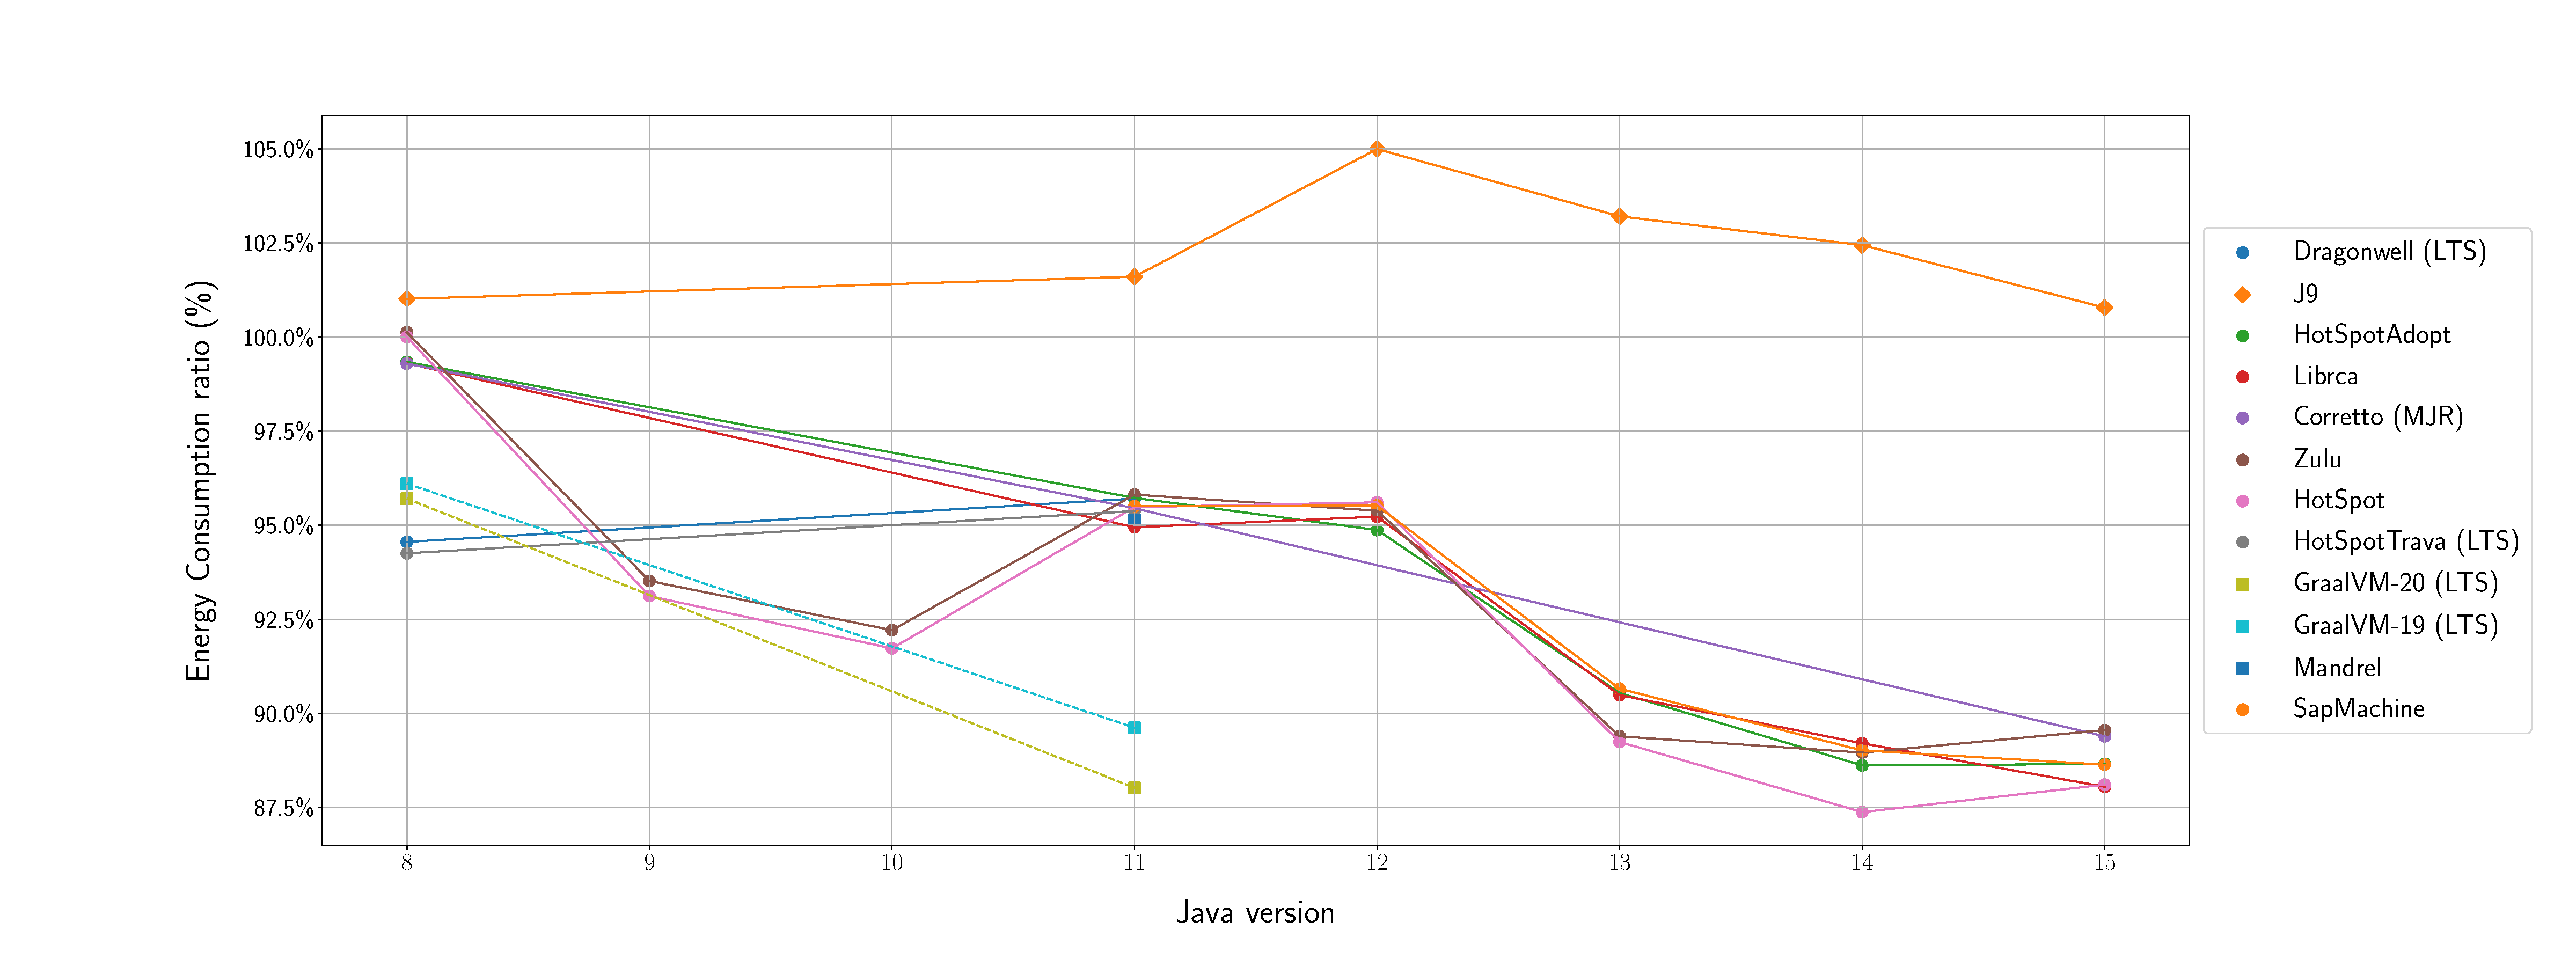
\includegraphics[width=\linewidth]{imgs/alljvms_chetemi8_baseon8.pdf}
    \caption{Energy consumption evolution of selected JVM distributions along versions.}
    \label{fig:JVMs}
\end{figure*}

One can observe that, along with time and versions, the energy efficiency of JVM distributions tends to improve (10\% savings), thus demonstrating the benefits of optimizations delivered by the communities.
Yet, one can also observe that energy consumption may differ from one distribution to another, thus showing that the choice of a JVM distribution may have a substantial impact on the energy consumption of the deployed software services.
For example, one can note that \textsc{J9} can exhibit up to 15\% of energy consumption overhead, while other distributions seem to converge towards a lower energy footprint for the latest version of Java.
As \textsc{GraalVM} adopts a different strategy focused on LTS support, one can observe that its recent releases provide the best energy efficiency for Java\,11, but recent releases of other distributions seem to reach similar efficiency for Java\,13 and above, which are recent versions not supported by \textsc{GraalVM} yet.

Interestingly, this convergence of distributions has been observed since Java\,11 and coincides with the adoption of DCE\,VM by \textsc{HotSpot}.
Ultimately, 3 clusters of JVMs that encompass JVMs with similar energy consumption can be seen through \Cref{fig:JVMs}: \textsc{J9}, the \textsc{HotSpot} and its variants, and \textsc{GraalVM}.
Additional detailed figures to illustrate the evolution of energy consumption per benchmark/JVM are made available from the online repository.\footnote{\url{https://github.com/chakib-belgaid/jvm-comparaison}}

Then, \Cref{fig:hotspot8} depicts the evolution of the energy consumption of the $12$ benchmarks, when executed on the \textsc{HotSpot} JVM.
\Cref{fig:hotspot8} reports on the energy consumption variation of individual benchmarks, using \textsc{HotSpot-8}\ as the baseline.
Our results show that the JVM version can severely impact the energy consumption of the application.
However, unlike \Cref{fig:JVMs}, one can observe that, depending on applications, the latest JVM versions can consume less energy (60\% less energy for \textsf{Scrabble}) or more energy (25\% more energy for the \textsf{Neo4J}).
It is worth noticing that the energy consumption of some benchmarks, such as \textsf{Reactors}, exhibit large variations across JVM versions due to experimental features and changes that are not always kept when releasing LTS versions (version 11 here).
For example, the introduction of \texttt{VarHandle} to allow low-level access to the memory order modes available in JDK 9~\footnote{\url{https://gee.cs.oswego.edu/dl/html/j9mm.html}} and work along \texttt{Unsafe Class} was removed from JVM 11.\footnote{\url{https://blogs.oracle.com/javamagazine/the-unsafe-class-unsafe-at-any-speed}}

\begin{figure*}%[ht]
    \centering
    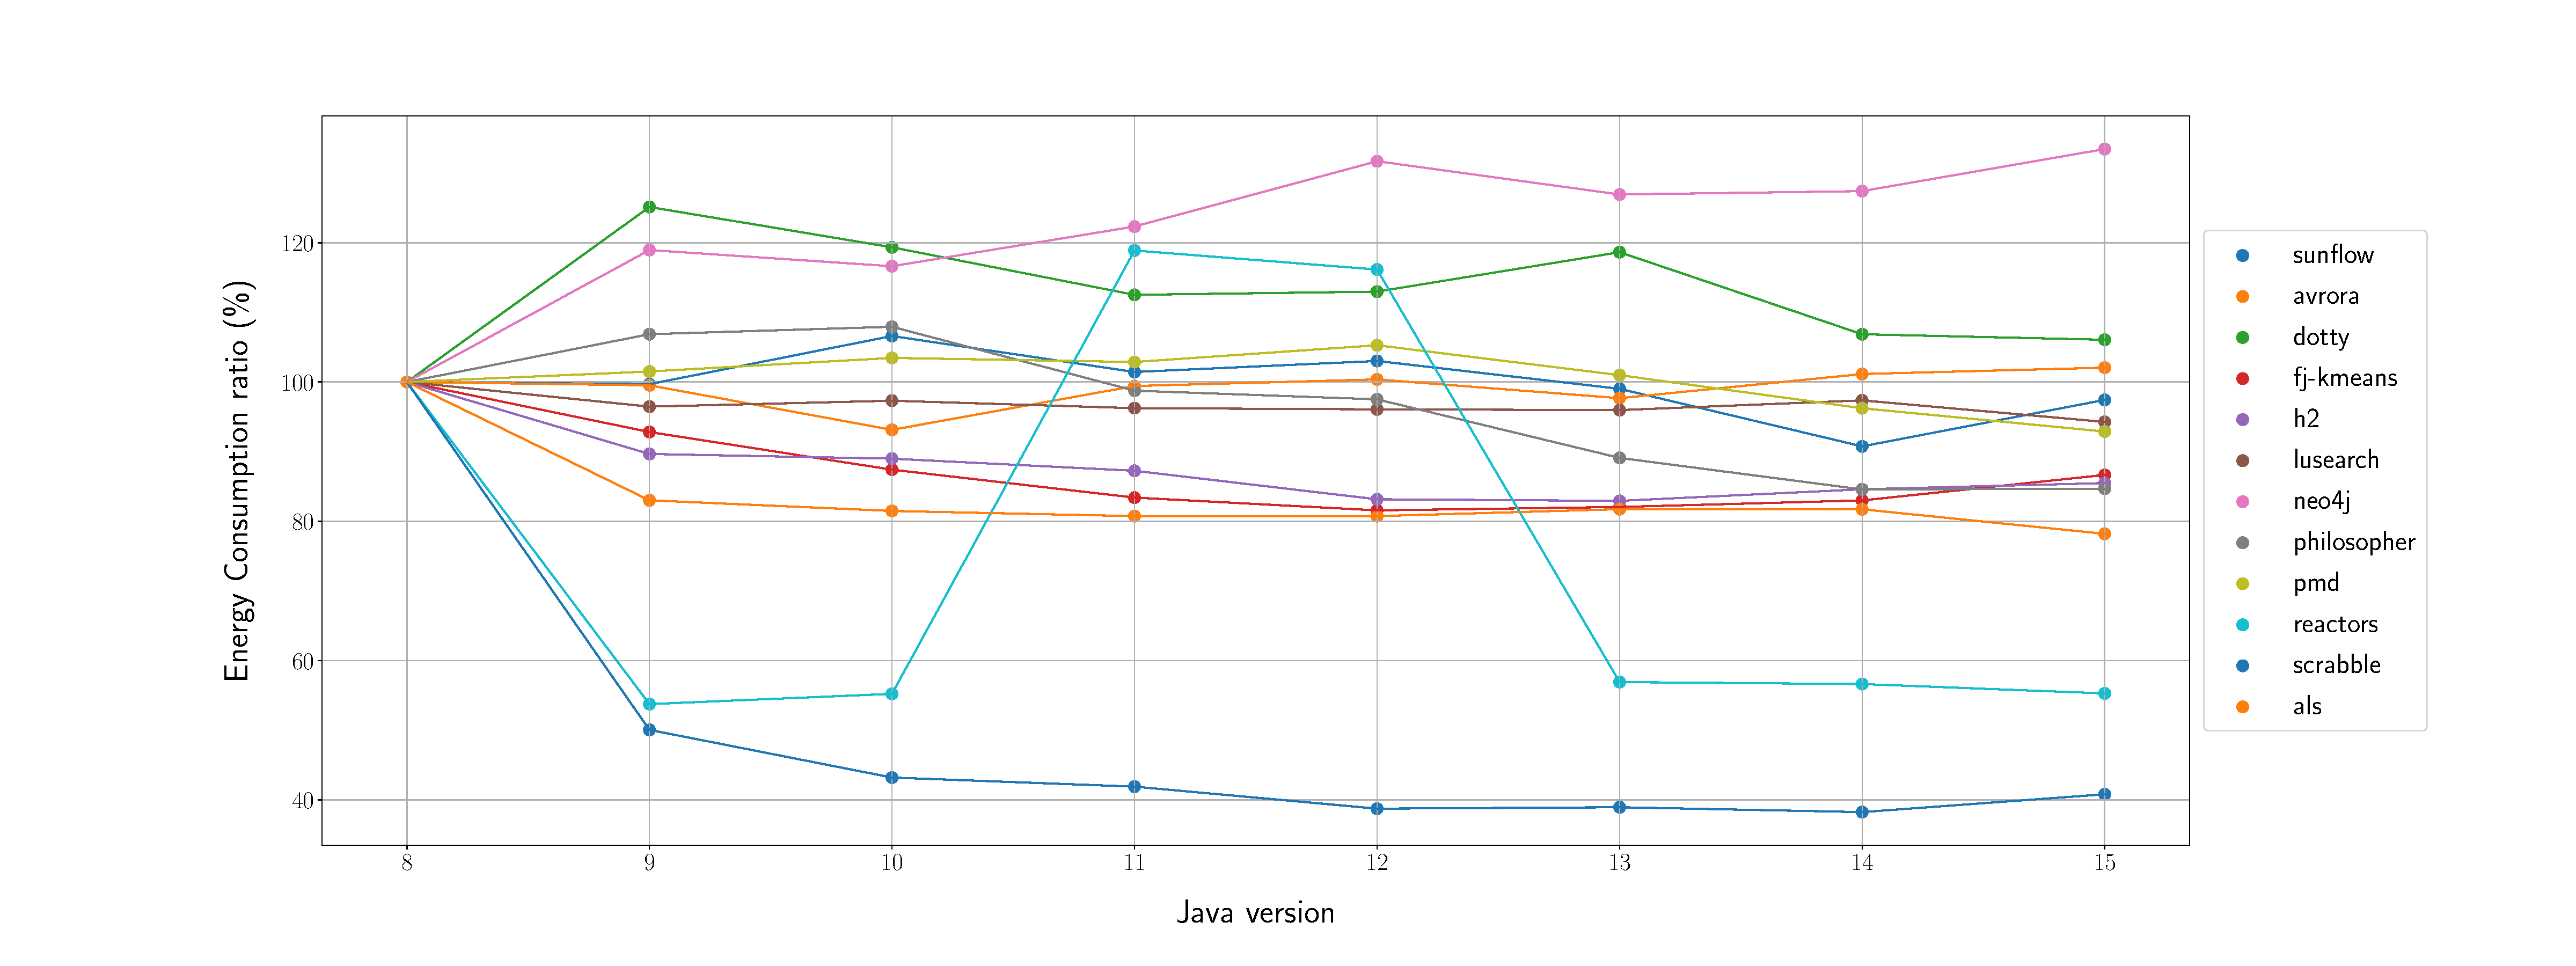
\includegraphics[width=\linewidth]{imgs/lineplothotspot_chetemi8_baseon8}
    \caption{Energy consumption of the HotSpot JVM along versions.}
    \label{fig:hotspot8}
\end{figure*}

% The purpose of this experiment is to check whether the JVM choice can affect the energy consumption of software.
% Yet, the purpose is also to retrieve some mainline information on the JVMs in order to achieve a better energy efficiency.
% Figures \ref{avrora} and \ref{scrabble} depict examples of the energy consumption end execution time of the Avrora and ALS benchmarks respectively.
% We noticed that many of the tested JVMs exhibit similar behaviors and consumption due to the high similarities between these versions.
% In fact, many versions share the same JVM core, and the differences between them are minor (sometimes just packaging changes from a constructor to another) to have any substantial impact in performance or energy consumption.

% \begin{figure*}%[ht]
% 	\begin{subfigure}{\textwidth}
% 		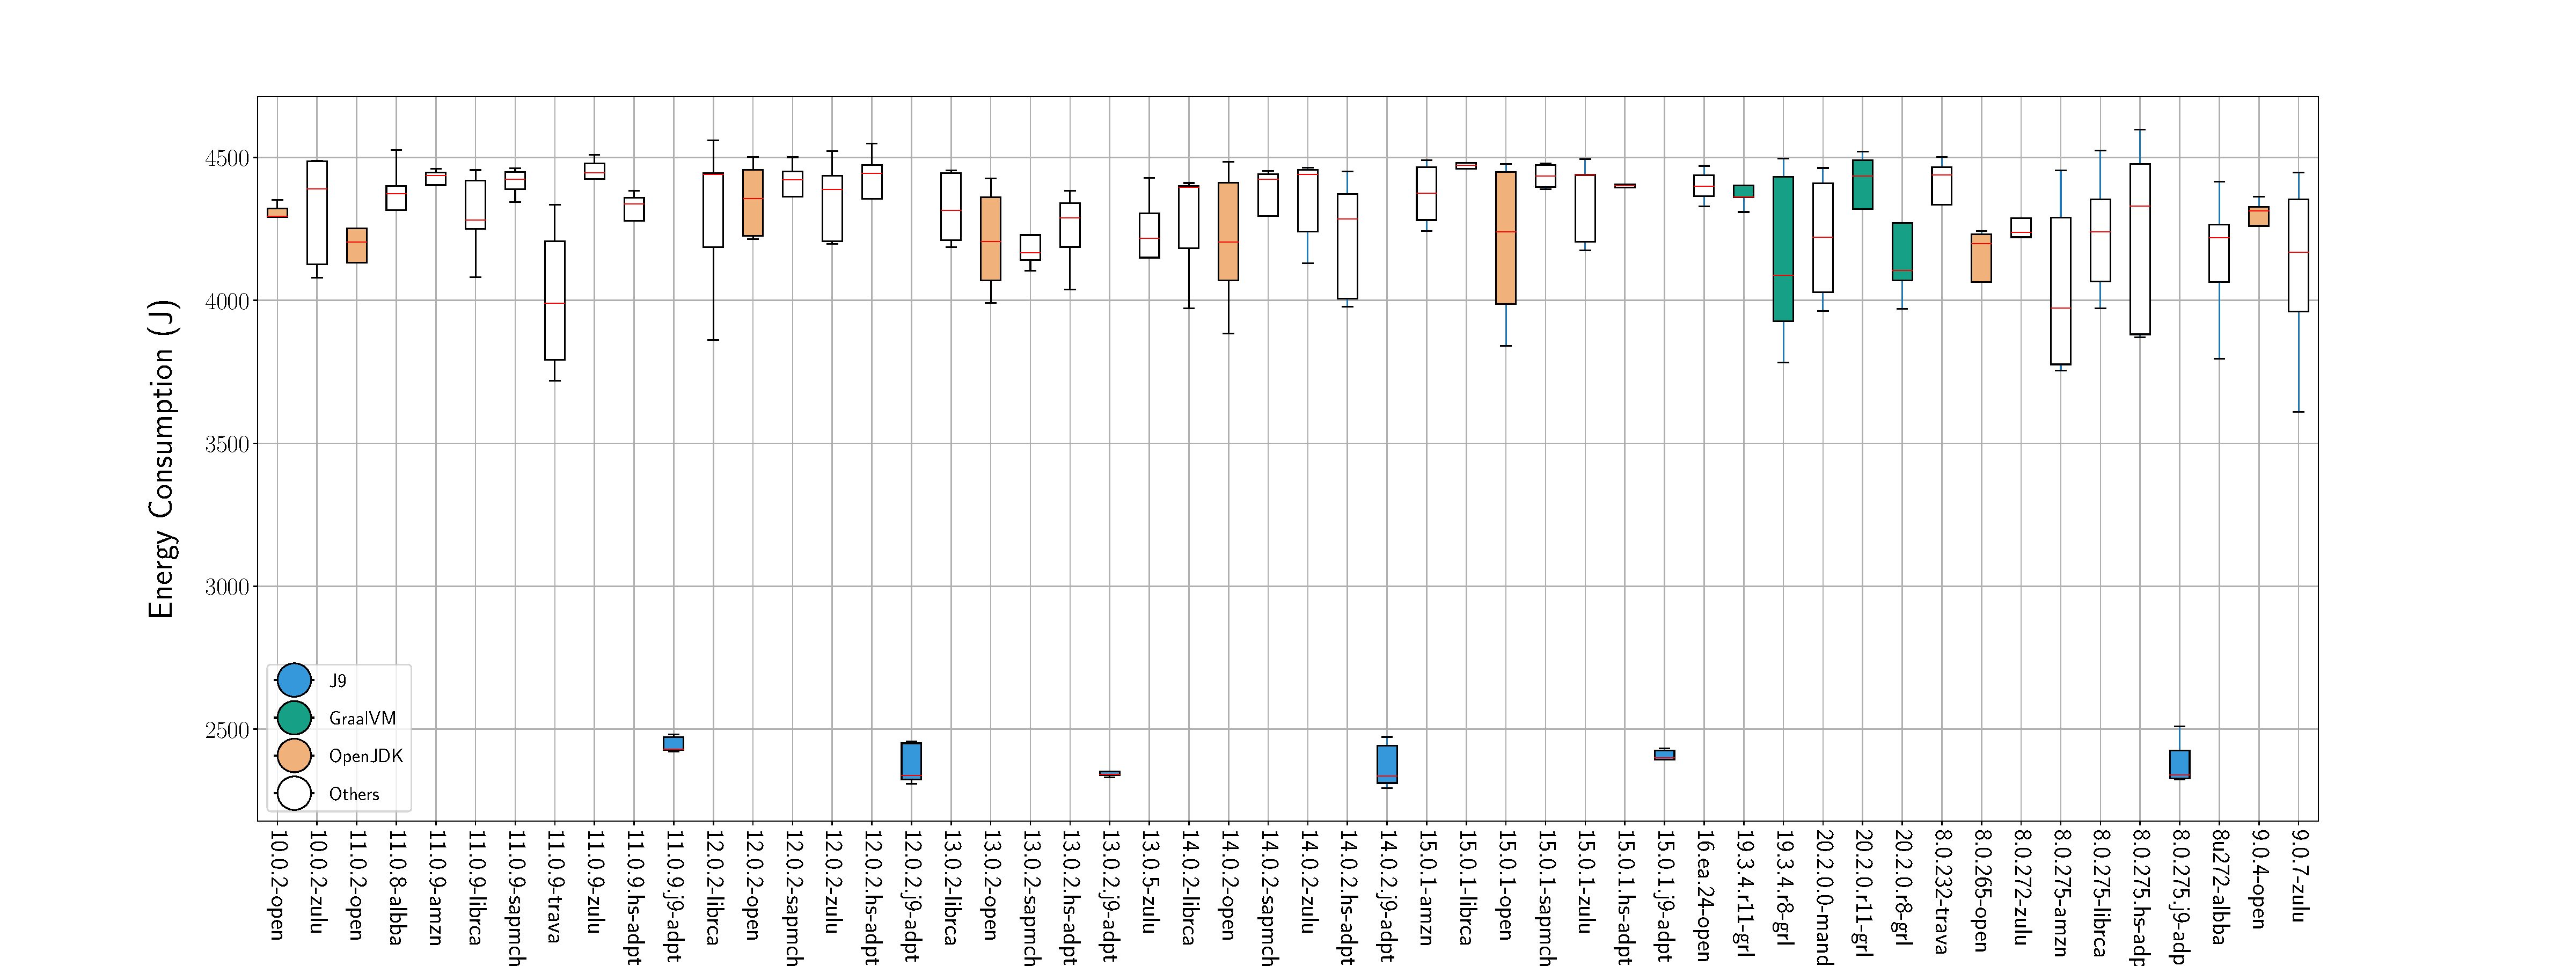
\includegraphics[width=\linewidth]{imgs/energy_pkg_all_avrorachetemi-8.pdf}
% 		\centering
% 		\captionsetup{justification=centering}
% 		\caption{Energy consumption of the Avrora benchmark using the 52 JVMs}\label{fig:avrora_energy}
% 	\end{subfigure}
% 	\begin{subfigure}{\textwidth}
% 		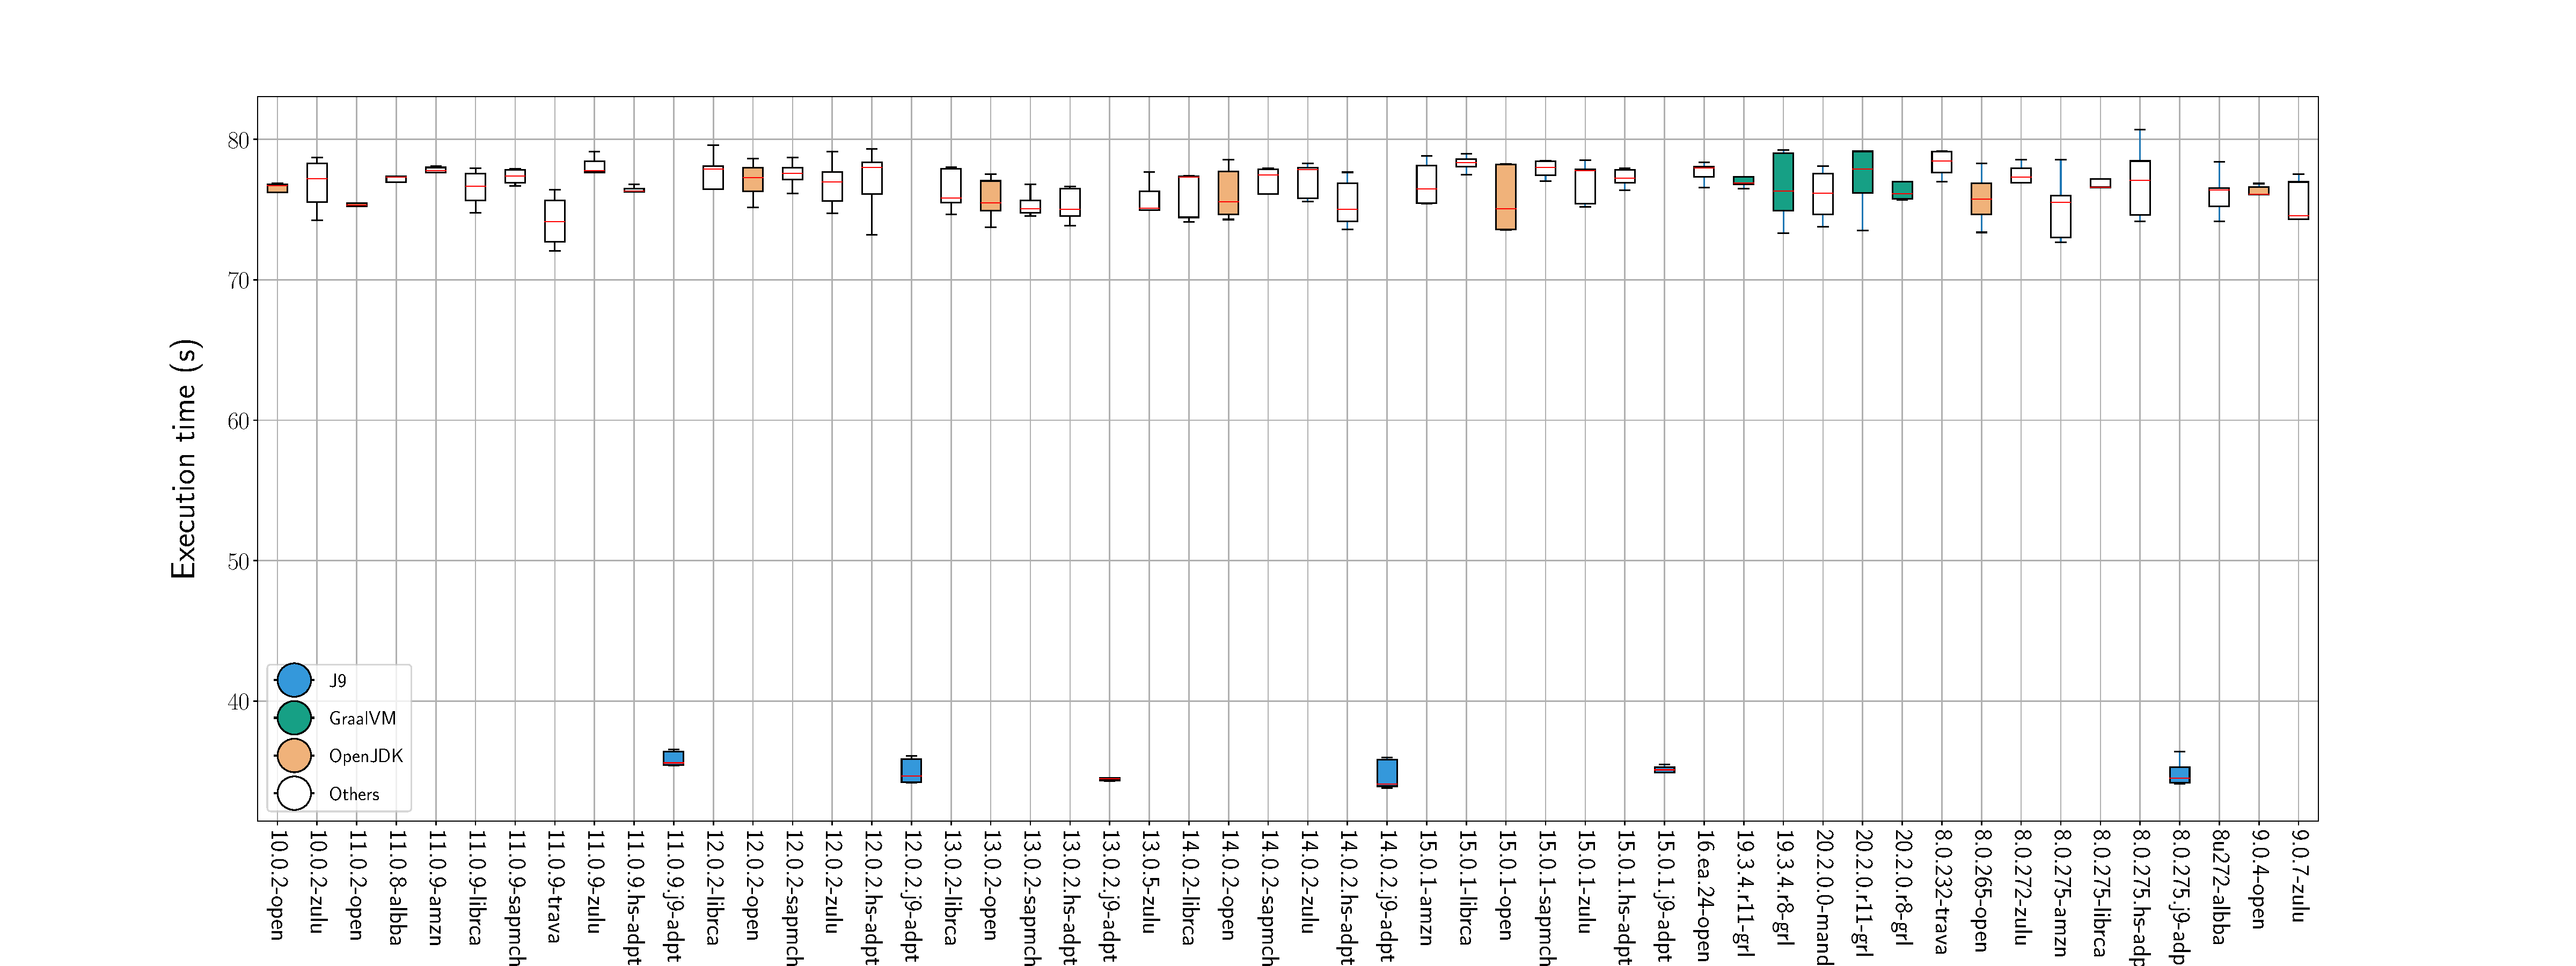
\includegraphics[width=\linewidth]{imgs/execution_time_all_avrorachetemi-8}
% 		\centering
% 		\captionsetup{justification=centering}
% 		\caption{Execution time of the Avrora benchmark using the 52 JVMs}\label{fig:avrora_time}
% 	\end{subfigure}
% 	\caption{Energy consumption and execution time of the Avrora benchmark using the 52 JVMs}
% 	\label{fig:avrora}
% \end{figure*}

% 	\begin{figure*}%[ht]
% 	\begin{subfigure}{\textwidth}
% 		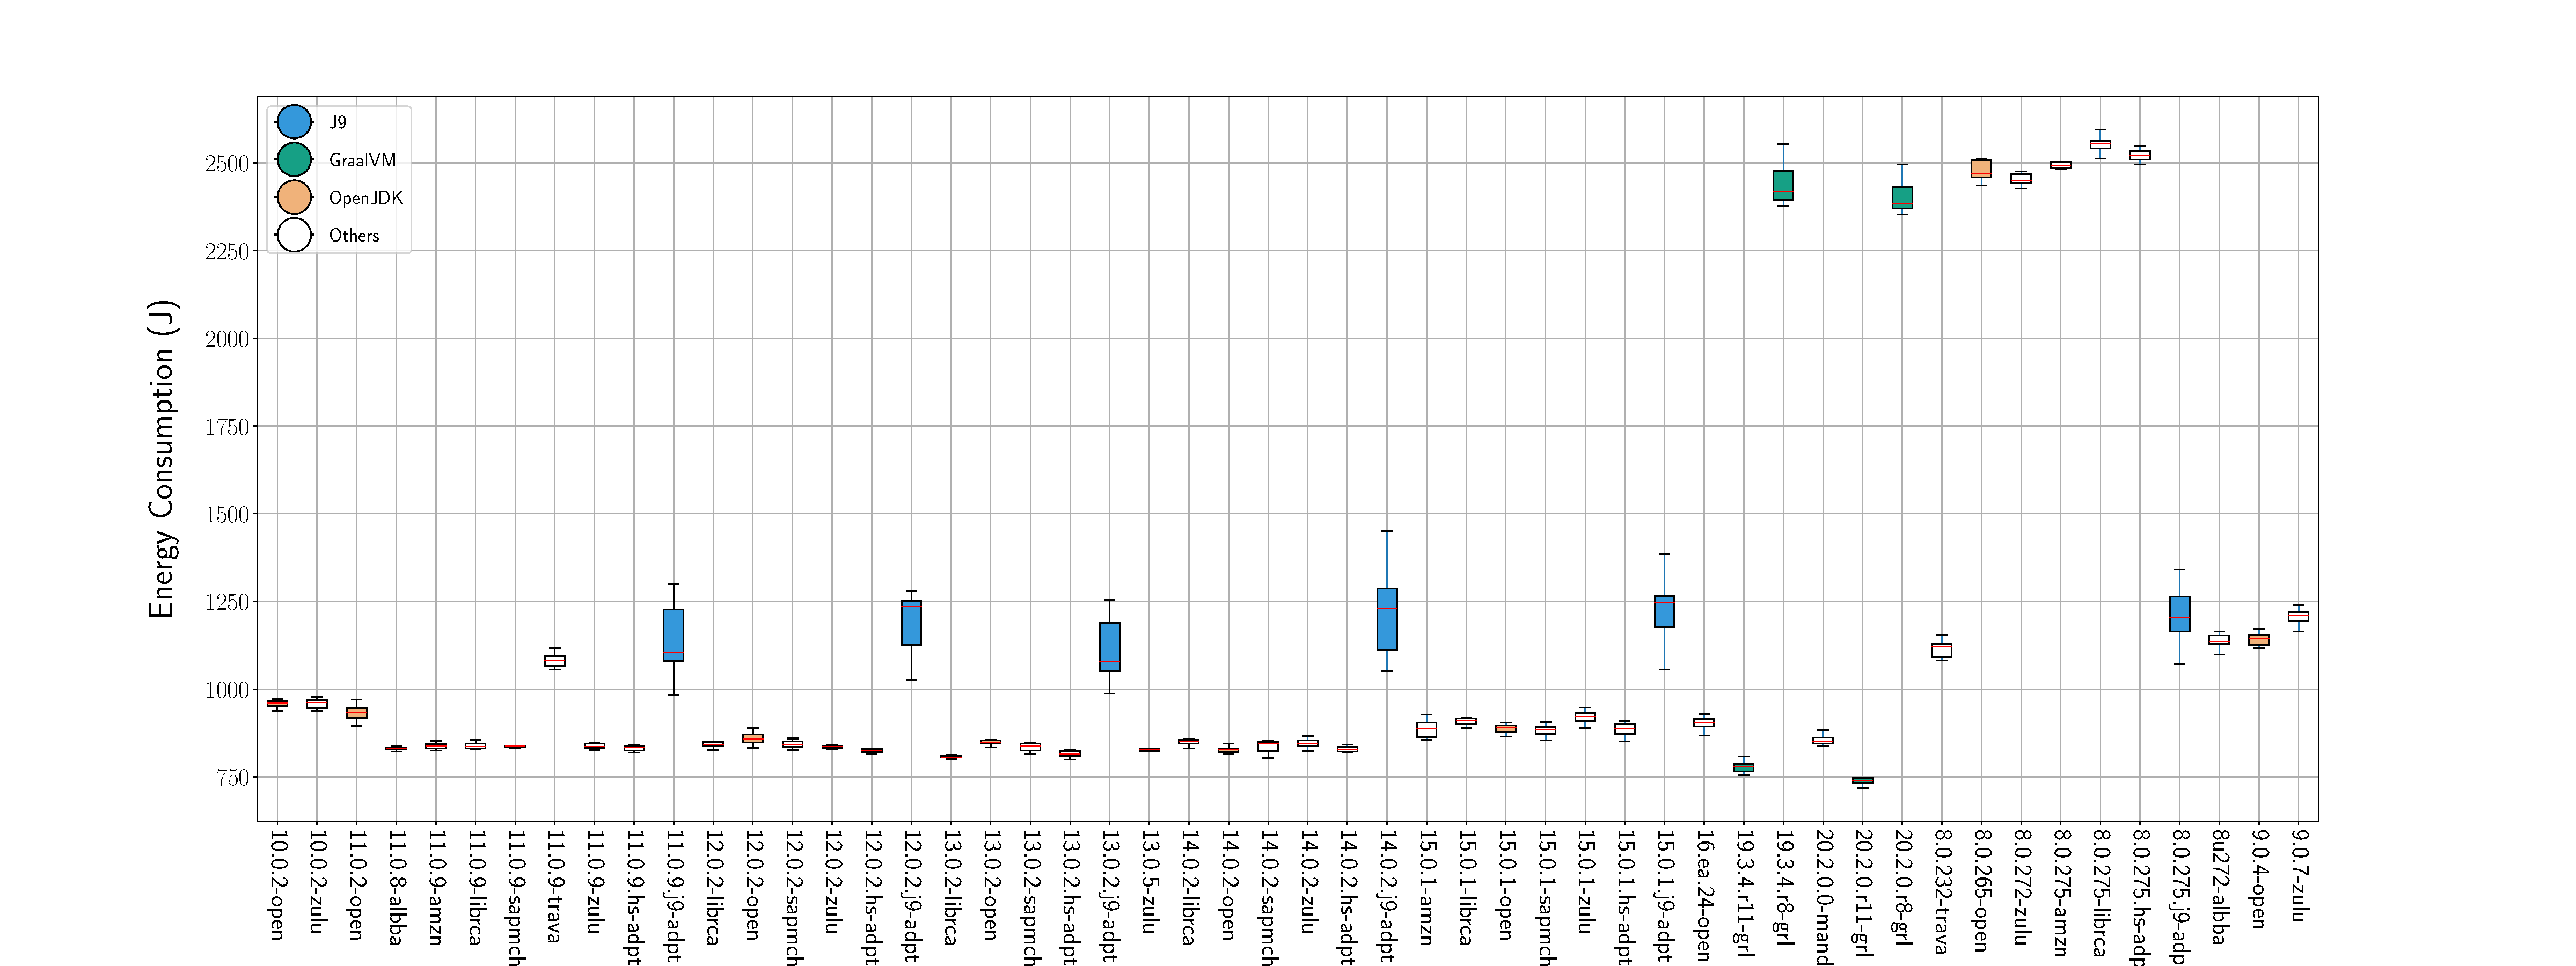
\includegraphics[width=\linewidth]{imgs/energy_pkg_all_scrabblechetemi-8.pdf}
% 		\centering
% 		\captionsetup{justification=centering}
% 		\caption{Energy consumption of the Scrabble benchmark using the 52 JVMs}\label{fig:scrabble_energy}
% 	\end{subfigure}
% 	\begin{subfigure}{\textwidth}
% 		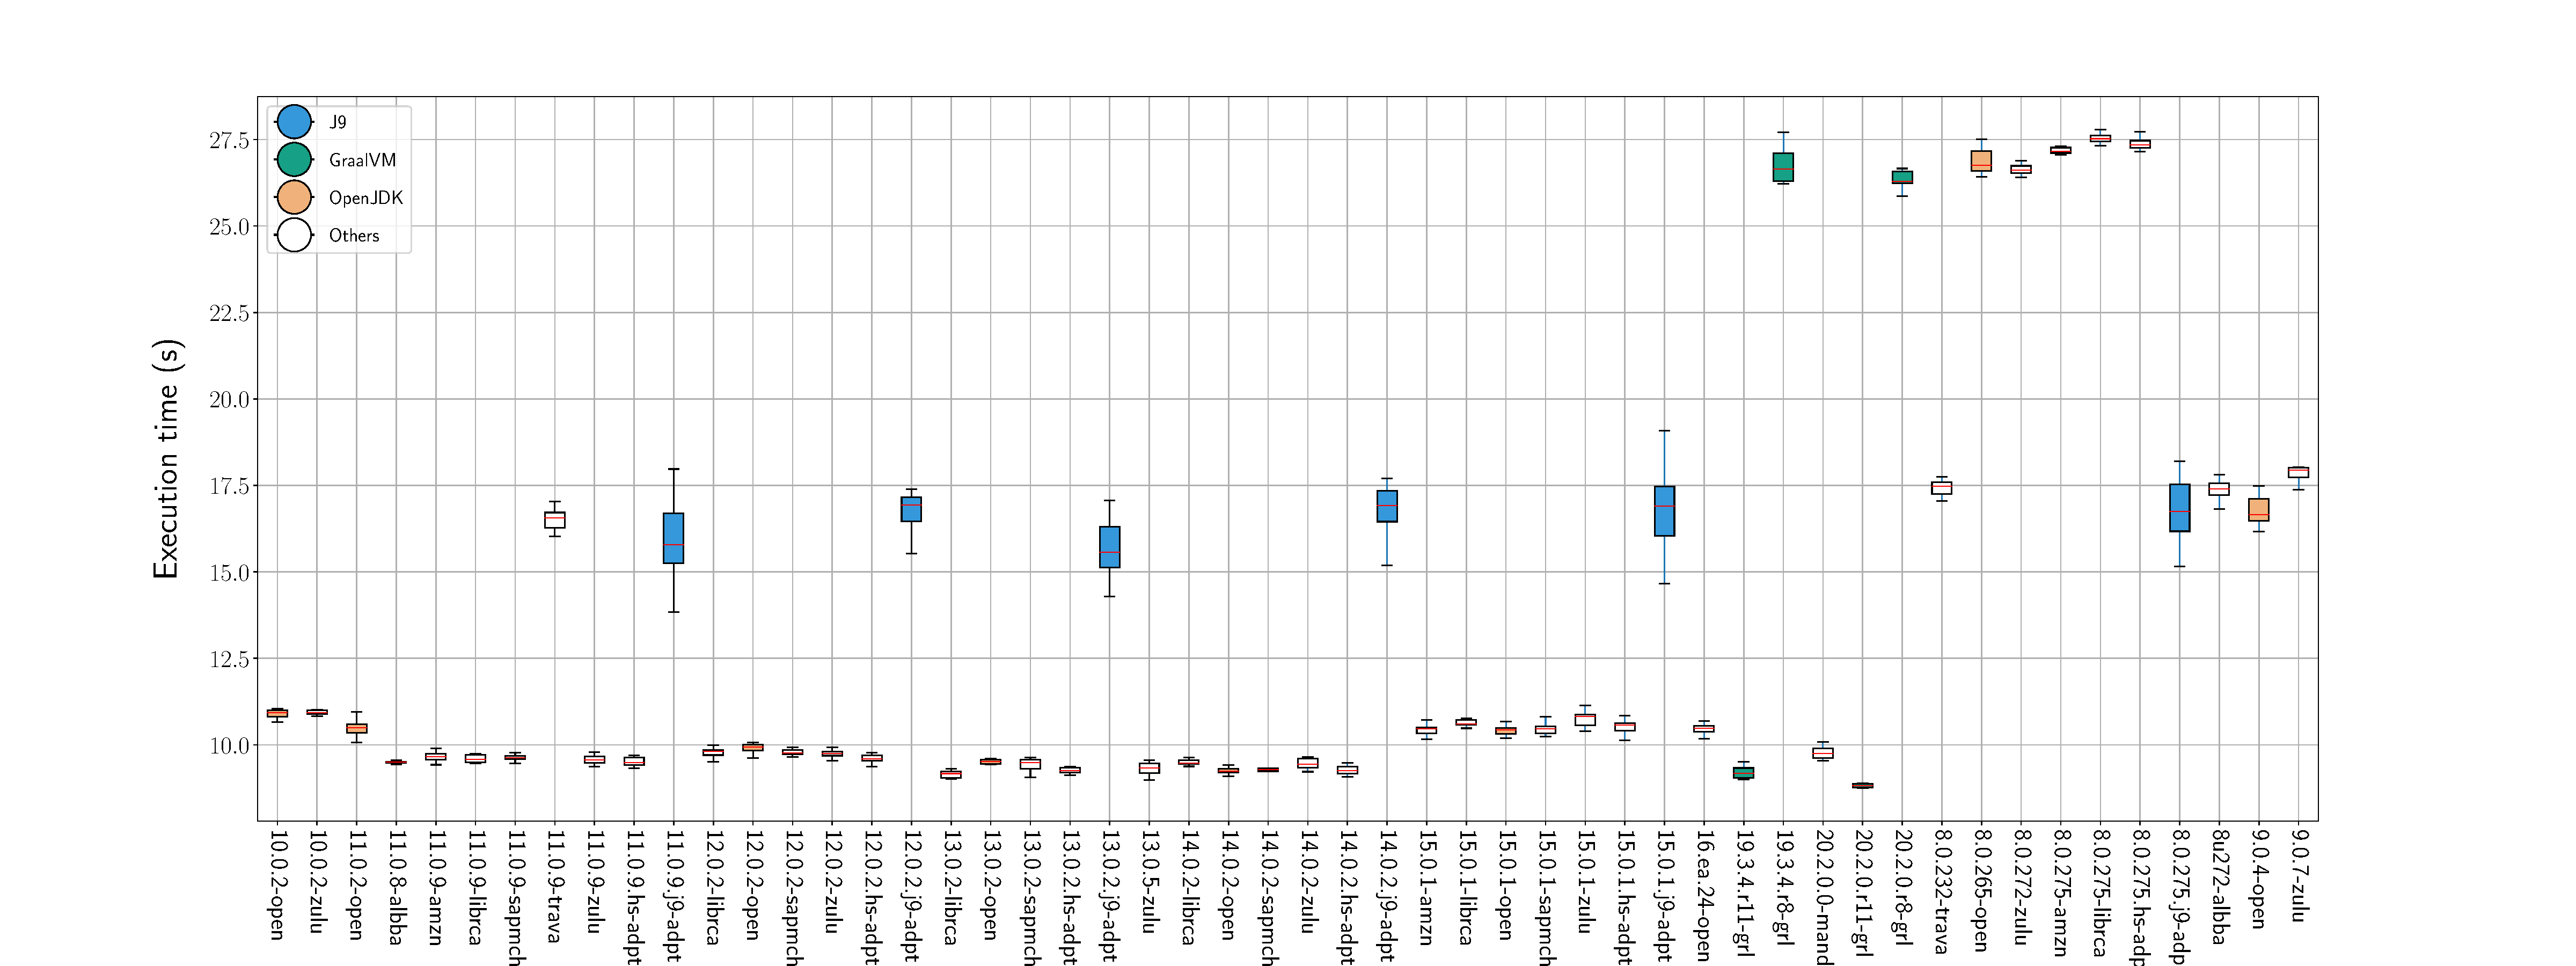
\includegraphics[width=\linewidth]{imgs/execution_time_all_scrabblechetemi-8}
% 		\centering
% 		\captionsetup{justification=centering}
% 		\caption{Execution time of the Scrabble benchmark using the 52 JVMs}\label{fig:scrabble_time}
% 	\end{subfigure}
% 	\caption{Energy consumption and execution time of the Scrabble benchmark using the 52 JVMs}
% 	\label{fig:scrabble}
% \end{figure*}

% We applied those comparison experiments on the whole benchmark set.
% The full results can be found through the anonymous link[footnote].
% Hence, Only 2 JVMs  gave energy consumption results that are different enough to be distinguished from the OpenJDK (GraalVM and J9).

Given that the wide set of distributions and versions seems to highlight 3 classes of energy behaviors, the remainder of this chapter considers the following distributions as relevant samples of JVM to be further evaluated: \textsf{20.2.0.r11-grl} (\textsc{GraalVM}), \textsf{15.0.1-open} (\textsc{HotSpot-15}), \textsf{15.0.21.j9} (\textsc{J9}).
We also decided to keep the \textsf{8.0.275-open} (\textsc{HotSpot-8}) as a baseline JVM for some figures to highlight the evolution of energy consumption over time/versions.

\Cref{fig:all_benchs} further explores the comparison of energy efficiency of the JVM distributions per benchmark.
One can observe that, depending on the benchmark's focus, the energy efficiency of JVM distributions may strongly vary.
When considering individual benchmarks, \textsc{J9} performs the worst for at least 6 out of 12 benchmarks---\emph{i.e.}, the worst ratio among the 4 tested distributions.
Even though, \textsc{J9} can still exhibit a significant energy saving for some benchmarks, such as \textsf{Avrora}, where it consumes 38\% less energy than \textsc{HotSpot} and others.

\begin{figure*}%[ht]
    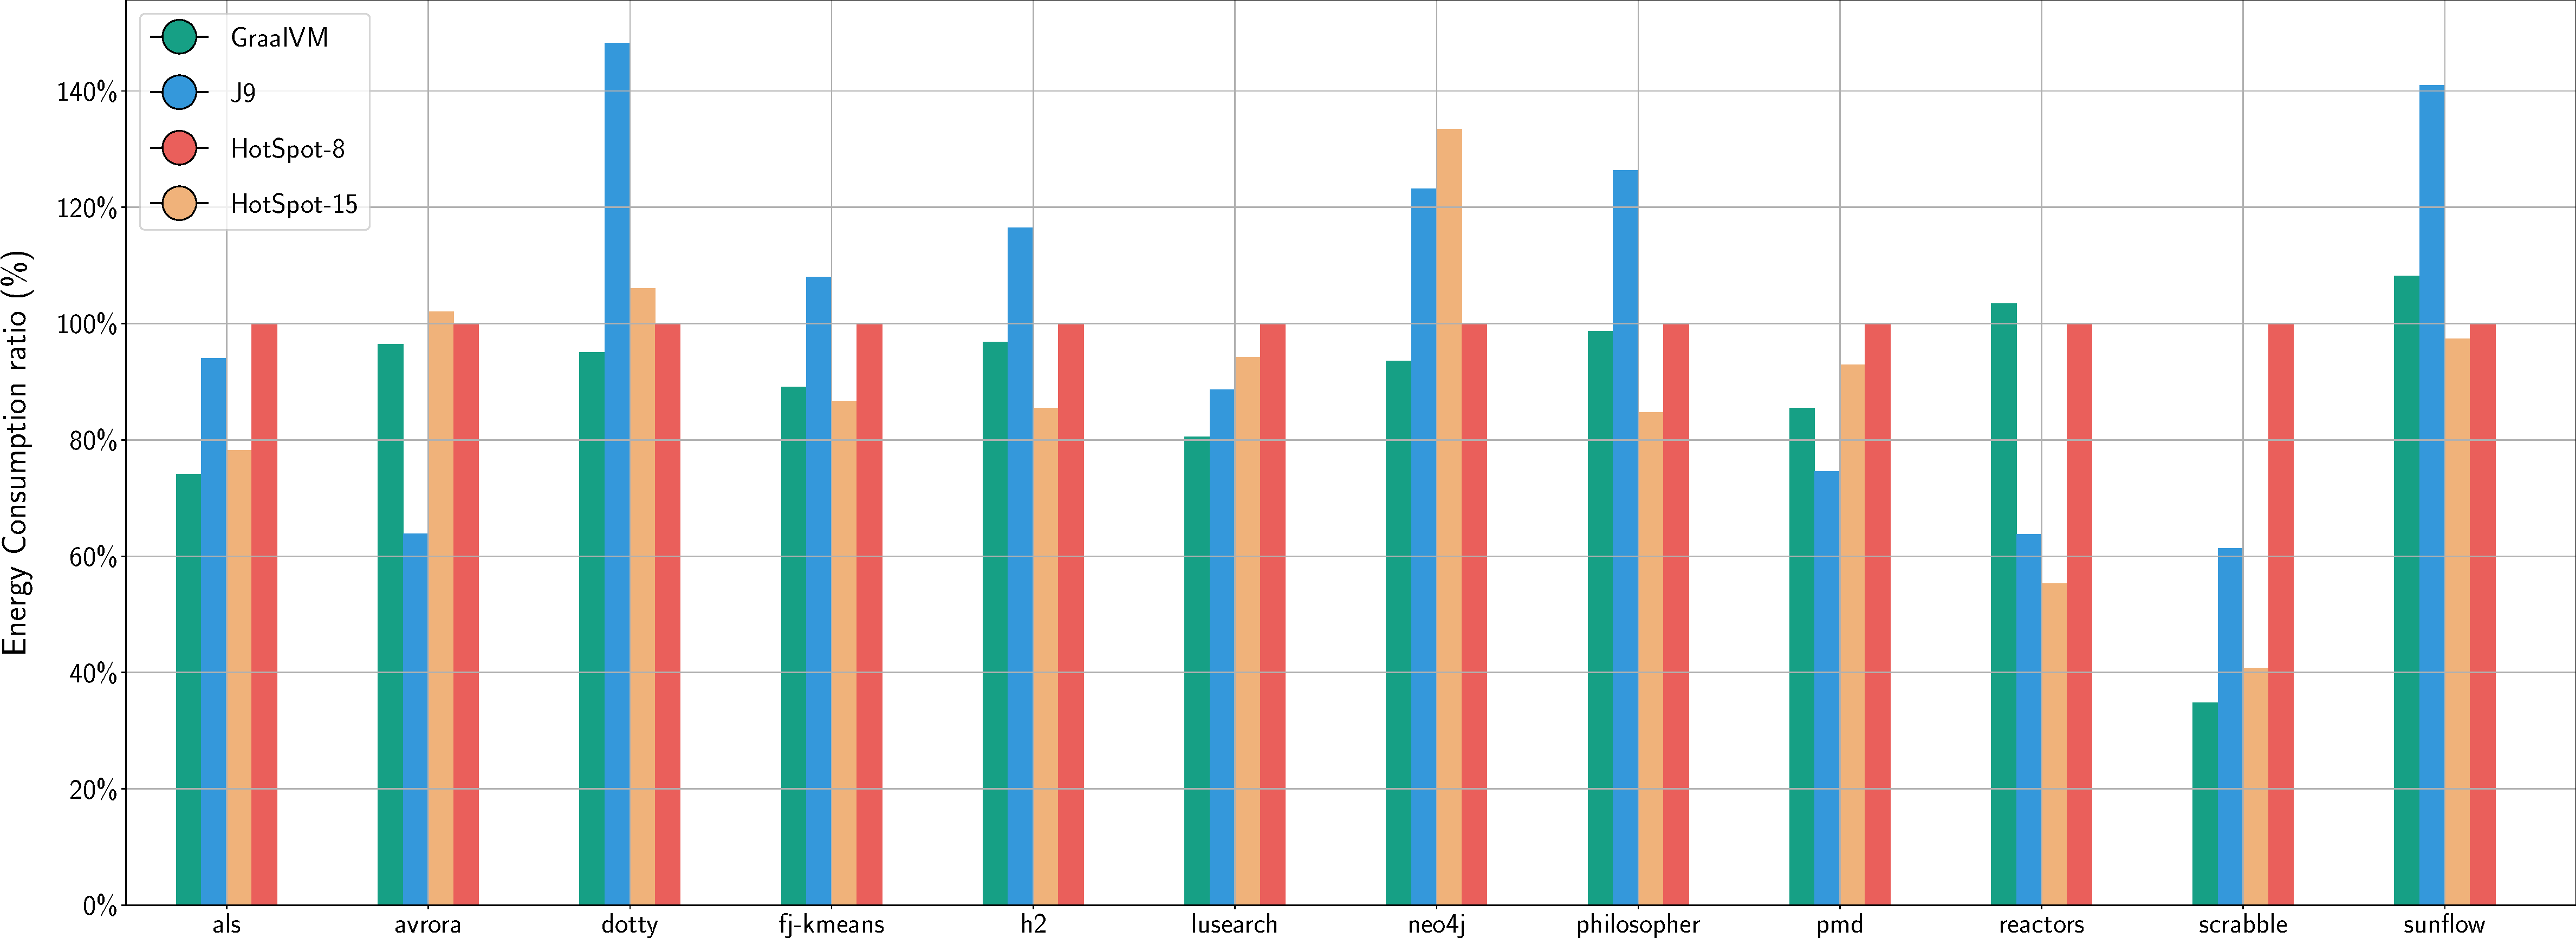
\includegraphics[width=.87\linewidth]{imgs/bar_plot_all_basedon8}
    \centering
    \captionsetup{justification=centering}
    \caption{Energy consumption comparison across Java benchmarks for \textsc{HotSpot}, \textsc{GraalVM} \& \textsc{J9}.}
    \label{fig:all_benchs}
\end{figure*}

Interestingly, \textsc{GraalVM} delivers good results overall, being among the distributions with low energy consumption for all benchmarks, except for \textsf{Reactors} and \textsf{Avrora}.
Yet, some differences still can be observed with \textsc{HotSpot} depending on applications.
The newer version of \textsc{HotSpot-15} was averagely good and, compared to \textsc{HotSpot-8}, it significantly enhances energy consumption for most scenarios.
Finally, \textsf{Neo4J} is the only selected benchmark where \textsc{HotSpot-8} is more energy efficient than \textsc{HotSpot-15}.


% We can clearly see through the previous figures \ref{avrora} and \ref{scrabble} that choosing OpenJDK, J9 or GraalVM can have a substantial impact the energy consumption and the execution time.
% % also it is still wildy used 
% In figure \ref{avrora}, the consumed energy to run the Avrora benchmark is 44\% less when using the J9 JVM.
% Moreover, we can even see that Avrora executions are running faster on J9 compared to the other platforms .
% In figure\ref{scrabble}, It is noticeable that the GraalVm with version 11 of Java is running 10\% faster and consuming 15\% less energy compared to other JVMs.


% These results can also be confirmed through many of the other benchmarks as each JVM can exhibit a better energy efficiency for some benchmarks and/or experiments.[ref to the footnote again].
% The results showed that we still can distinguish the 3 main platforms (OpenJDK, J9 and Graal) where noticeable energy consumption differences can be detected.
% Figure \ref{all_benchs} illustrates the ratio of consumed energy for the J9 and GraalVM platforms compared to OpenJDK 15.0.1.
% It clearly shows that the three JVM platforms rarely consume the same energy when running the same task,
% A platform can exhibit the best or worst performance/energy consumption depending the benchmark we tested.
% Overall, and among the 12 benchmarks we tested, GraalVM seemed to be the most interesting JVM energy-consumption wise.
% In fact, GraalVm is the most energy efficient in 5 of the 12 benchmarks, by up to 40\% for the Lusearch benchmark compared to OpenJDK.
% J9 on the other hand recorded the worst energy consumption for 7 of the 12 benchmarks. but gave some interesting results with ~45\% and ~25\% improvement for the Avrora and Pmd benchmarks respectively.
% This endorses the further investigation that has to be done in order to determine the different parameters that can contribute to this difference.
% While openJDK~15 and OpenJDK~8 often show close energy consumption (9 of the 12 benchmarks).
% However the oldest version of OpenJDK can consume half the energy consumption for some cases such as Neo4J, and up to ~80\% and ~130\% more for some other cases such as Reactors an Scrabble respectively.
% This proves that the later versions of OpenJDK doesn't essentially outperforms the older ones. 

% \paragraph{Energy Impact of JVM Distributions on services}
\vspace{6pt}
\noindent\textbf{Service-oriented applications.}
% The previous experiments have been conducted on deterministic jobs where we measured the energy consumption of many runs.
In this section, instead of considering bounded execution of benchmarks, we run the same benchmarks as services for 20 minutes, and we compare the average power and total requests processed by each of the 3 JVM distributions.
Globally, the results showed that the average power when using \textsc{GraalVM}, \textsc{HotSpot}, and \textsc{OpenJ9} is often equivalent and stable over time.
This means that the energy efficiency observed for some JVM distributions with job-oriented applications is mainly related to shorter execution times, which incidentally results in energy savings.
Nonetheless, we can highlight two interesting observations for two benchmarks whose behaviors differ from others.
First, the analysis of the \textsf{Scrabble} benchmark experiments showed that, in some scenarios, some JVMs can exhibit different power consumptions.
\Cref{fig:servicescrabble} depicts the power consumed by the 3 JVM distributions for the \textsf{Scrabble} benchmark.
One can clearly see that \textsc{GraalVM} requires an average power of 109\,W, which is 9\,W higher than \textsc{HotSpot-15} and 15\,W higher than \textsc{J9}.
% This average power consumption is stable over time.
When it comes to the number of requests processed by \textsf{Scrabbles} during that same amount of time, \textsc{GraalVM} completes $5,336$ requests, against $3,595$ for \textsc{HotSpot} and $2,603$ for \textsc{J9}, as shown in \Cref{table:power/request}.
The higher power usage for \textsc{GraalVM} helped in achieving a high amount of requests, but also the fastest execution of every request, which was 40\% faster on \textsc{GraalVM}.
Thus, \textsc{GraalVM} was more energy efficient, even if it uses more power, which confirms the results observed in \Cref{fig:all_benchs} for this benchmark.

\begin{table}
    \centering
    \caption{Power per request for \textsc{HotSpot}, \textsc{GraalVM} \& \textsc{J9}.}
    \label{table:power/request}
    \small
    \begin{tabular}{|c|c|c|c|c|}
        \hline
        \textbf{Benchmark}            & \textbf{JVM}     & \textbf{Power\,(P)} & \textbf{Requests\,(R)} & $P/R\,\times\,10^{-3}$ \\
        \hline
        \hline
        \multirow{3}{*}{\sf Scrabble} & \textsc{GraalVM} & 109\,W              & \best 5,336\,req       & \best 20\,mW           \\
        \cline{2-5}
                                      & \textsc{HotSpot} & 98\,W               & 3,595\,req             & 27\,mW                 \\
        \cline{2-5}
                                      & \textsc{J9}      & \best 92\,W         & 2,603\,req             & 35\,mW                 \\
        \hline
        \multirow{3}{*}{\sf Dotty}    & \textsc{GraalVM} & \best 45\,W         & 510\,req               & 88\,mW                 \\
        \cline{2-5}
                                      & \textsc{HotSpot} & \best 45\,W         & \best 597\,req         & \best 75\,mW           \\
        \cline{2-5}
                                      & \textsc{J9}      & 46\,W               & 381\,req               & 120\,mW                \\
        \hline
    \end{tabular}
\end{table}

\begin{figure*}%[ht]
    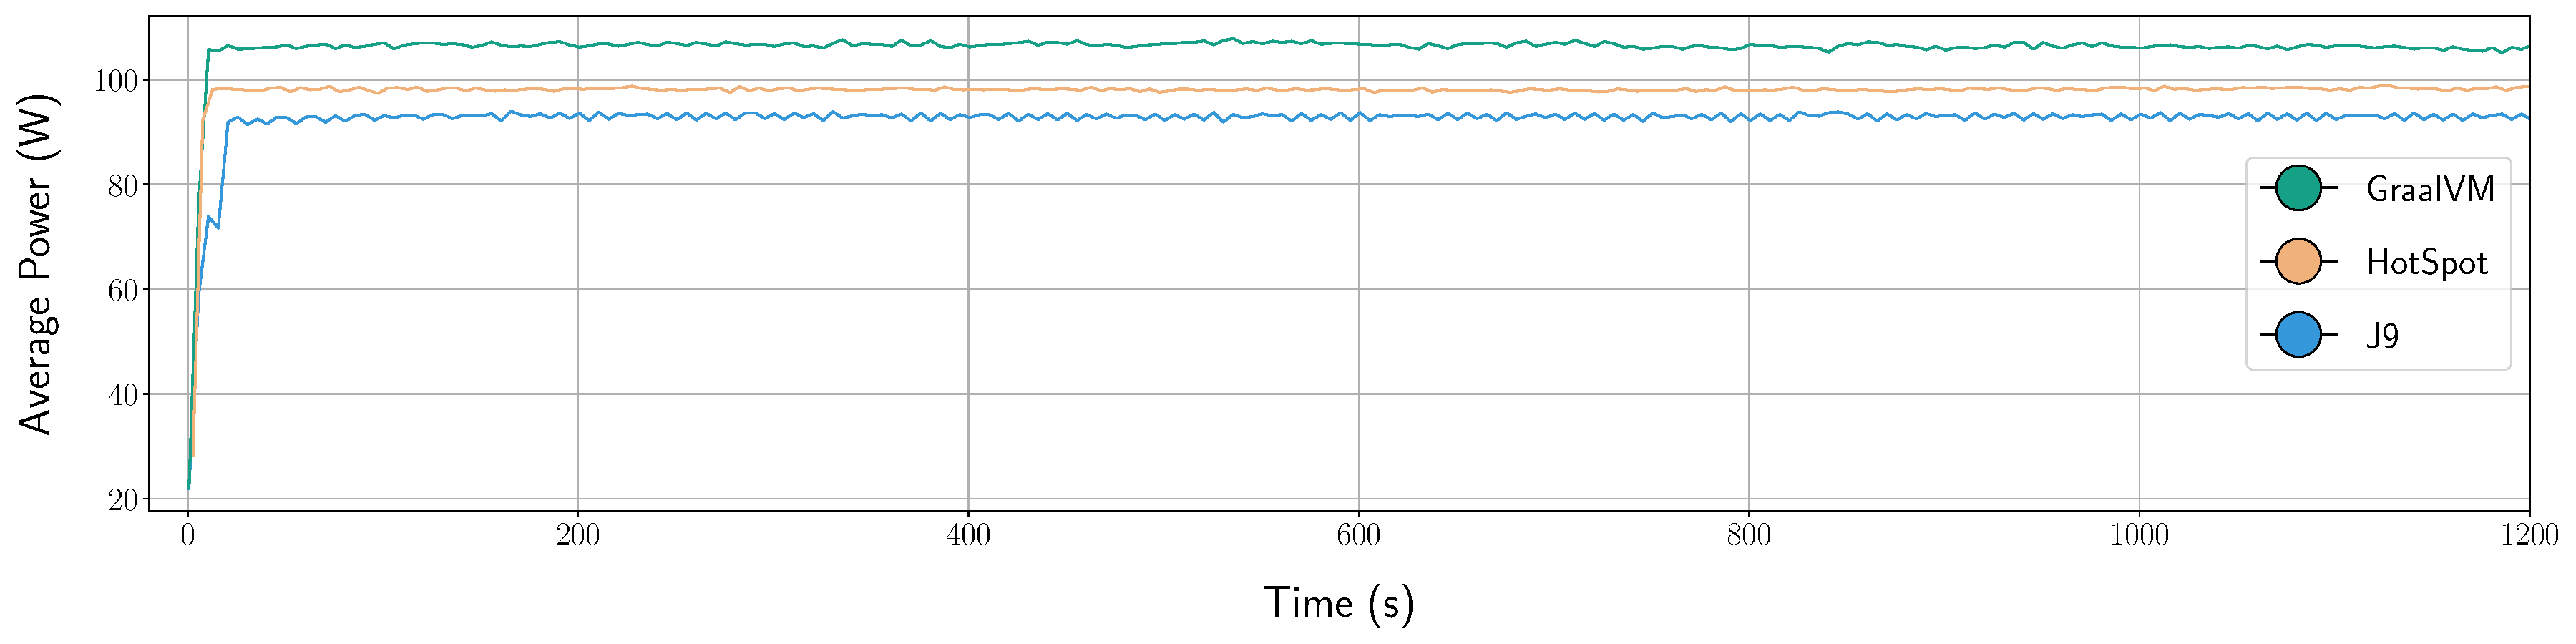
\includegraphics[width=.9\linewidth]{imgs/powers_chetemi-2-scrabble.pdf}
    \centering
    \captionsetup{justification=centering}
    \caption{Power consumption of \textsf{Scrabble} as a service for \textsc{HotSpot}, \textsc{GraalVM} \& \textsc{J9}.}
    \label{fig:servicescrabble}
\end{figure*}

The second interesting situation was observed on the \textsf{Dotty} benchmark.
More specifically, during the first $100$ seconds of the execution of the \textsf{Dotty} benchmark on all evaluated JVMs.
At the beginning of the execution, \textsc{GraalVM} has a slightly lower power consumption, is faster, and consumes 10\% less energy.
After about $150$ seconds, the power differences between the 3 JVMs is barely noticeable.
One can, however, notice the effect of the JIT, as \textsc{HotSpot} takes the advantage over \textsc{GraalVM} and becomes more energy efficient.
In total, \textsc{HotSpot} completes $597$ requests against $510$ for \textsc{GraalVM} and $381$ for \textsc{J9}, as shown in \Cref{table:power/request}.
\textsc{HotSpot} was thus the best choice in the long term, which explains why it is always necessary to consider a warm-up phase and wait for the JIT to be triggered before evaluating the effect of the JVM or the performance of an application.
This is precisely what we did in our experiments, and it is why \textsc{HotSpo}t was more energy efficient than \textsc{GraalVM} in \Cref{fig:all_benchs}; therefore, ignoring the warm-up phase would have been misleading.

\begin{figure*}%[ht]
    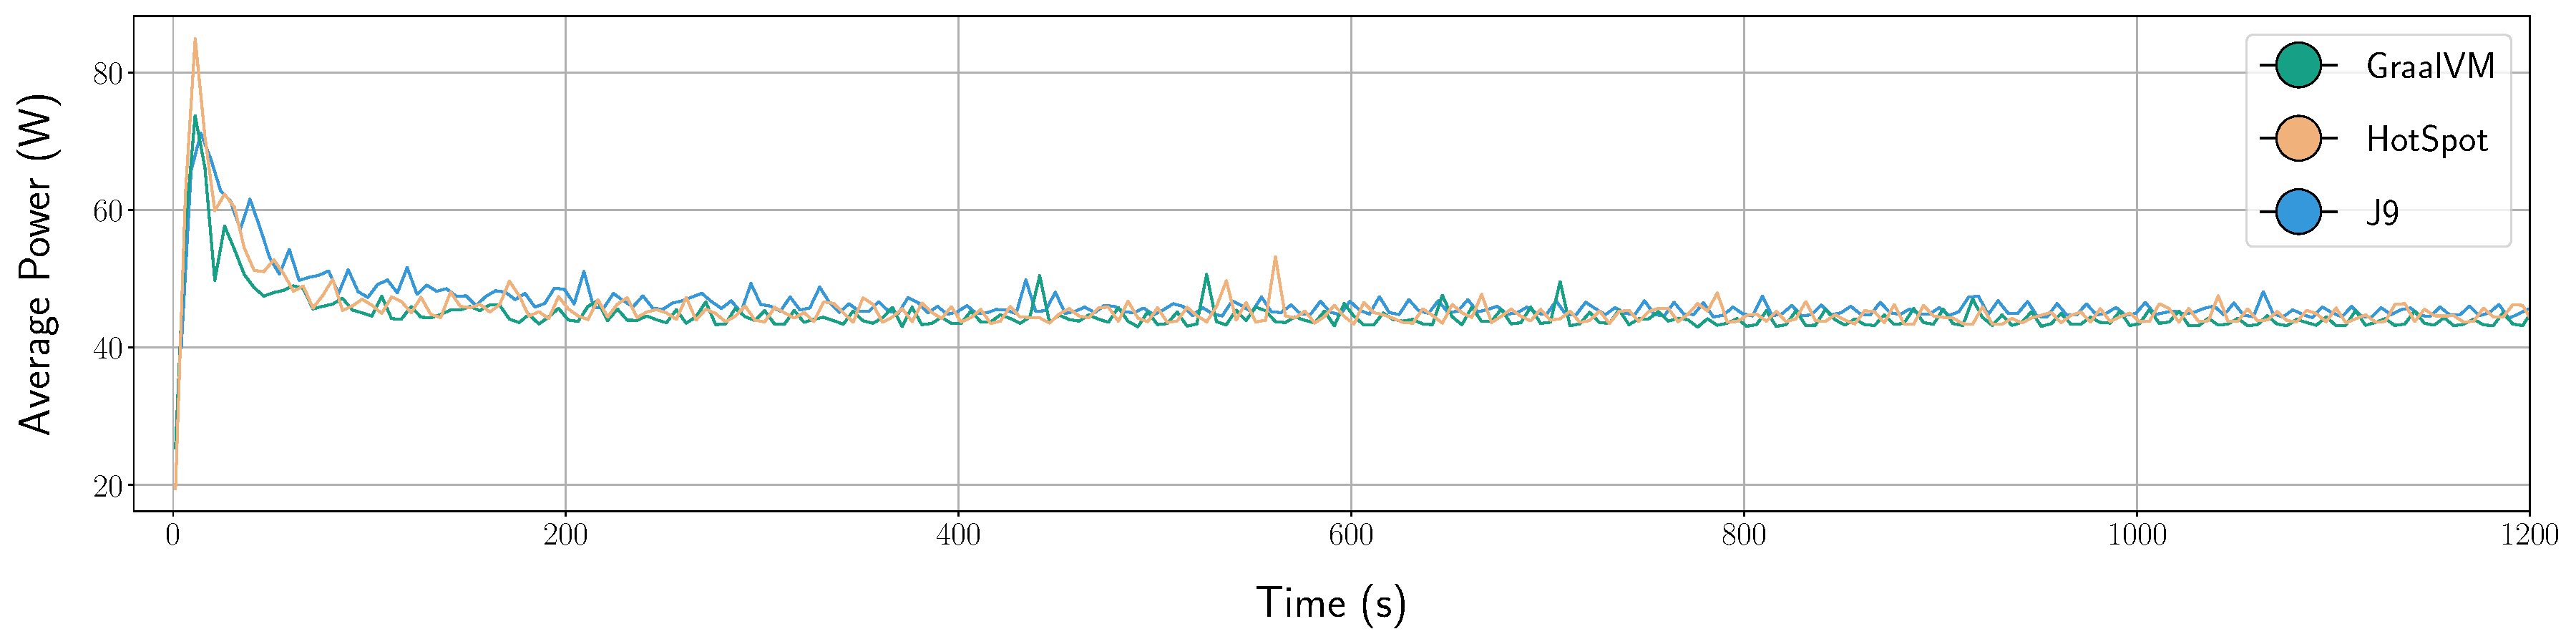
\includegraphics[width=.9\linewidth]{imgs/powers_chetemi-2-dotty.pdf}
    \centering
    \captionsetup{justification=centering}
    \caption{Power consumption of \textsf{Dotty} as a service for \textsc{HotSpot}, \textsc{GraalVM} \& \textsc{J9}.}
    \label{fig:servicedotty}
\end{figure*}
% \bigbreak
\begin{mdframed}[]
    To answer \textbf{RQ\,1}, we conclude that---while most of the JVM platforms perform similarly---we can cluster JVMs in 3 classes: \textsc{HotSpot}, \textsc{J9}, and \textsc{GraalVM}.
    The choice of one JVM of these classes can have a major impact on software energy consumption, which strongly depends on the application context.
    When it comes to the JVM version, the latest releases tend to offer the lowest power consumption, but experimental features should be carefully configured, thus further questioning the impact of JVM parameters.
\end{mdframed}

\subsection{Energy Impact of JVM Settings}
The purpose of our study is not only to investigate the impact of the JVM platform on energy consumption, but also the different JVM parameters and configurations that might have a positive or negative effect, with a focus on 3 available settings: multi-threading, JIT, and GC.

\subsubsection{Multithreading}
The purpose of this phase is to investigate the impact JVM thread management strategies on energy consumption.
This encompasses exploring if the management strategies of application-level parallelism (so-called \emph{threads}) result in different energy efficiencies, depending on JVM distributions.

Investigating such a hypothesis requires a selection of highly parallel and CPU-intensive benchmarks, which is one of the main criteria for our benchmark selection.
As no tool can accurately monitor the energy consumption at a thread level, we monitor the global power consumption and CPU utilization during the execution using RAPL for the energy, and several Linux tools for the CPU-utilization (\texttt{htop}, \texttt{cpufreq}).
%The experiments showed differences in energy consumption between the 3 JVMs and even between 2 version on the HotSpot VM.
Knowing that most of the benchmarks are multi-threaded jobs that use multiple cores, further analysis of thread management is required to understand the results of our previous experiments.
We thus selected the benchmarks that highlighted the highest differences along JVM distributions from \Cref{fig:all_benchs}, namely \textsf{Avrora} and \textsf{Reactors}.
We studied their multi-threaded behavior to optimize their energy efficiency.

\begin{figure*}%[ht]
    \begin{subfigure}{\textwidth}
        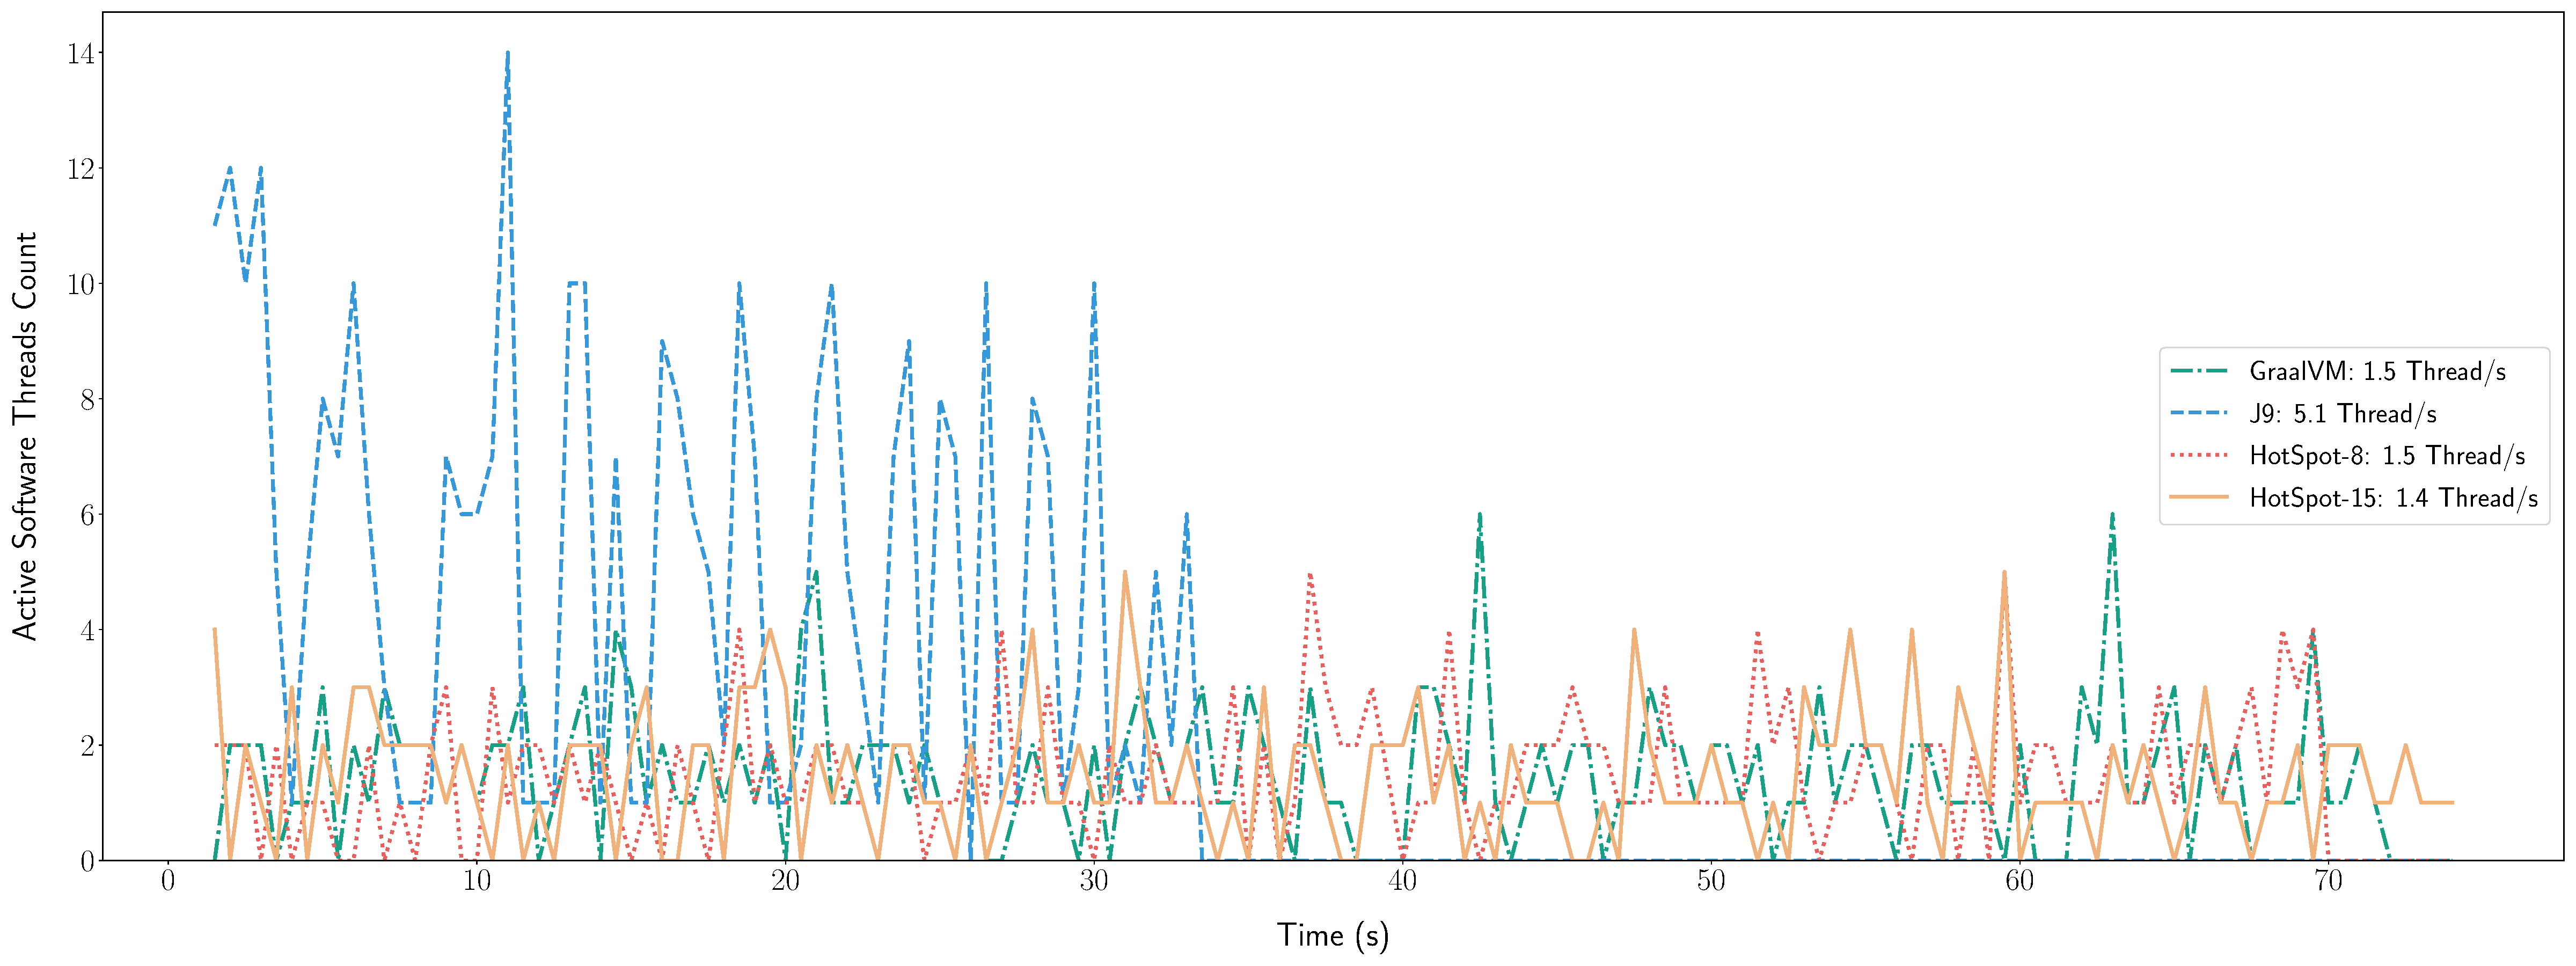
\includegraphics[width=.9\linewidth]{imgs/active_threads_avrora_chetemi_3}
        \centering
        \captionsetup{justification=centering}
        \caption{Active threads of \textsf{Avrora} when using \textsc{HotSpot}, \textsc{GraalVM}, or \textsc{J9}.}
        \label{fig:avrora_threads}
    \end{subfigure}
    \begin{subfigure}{\textwidth}
        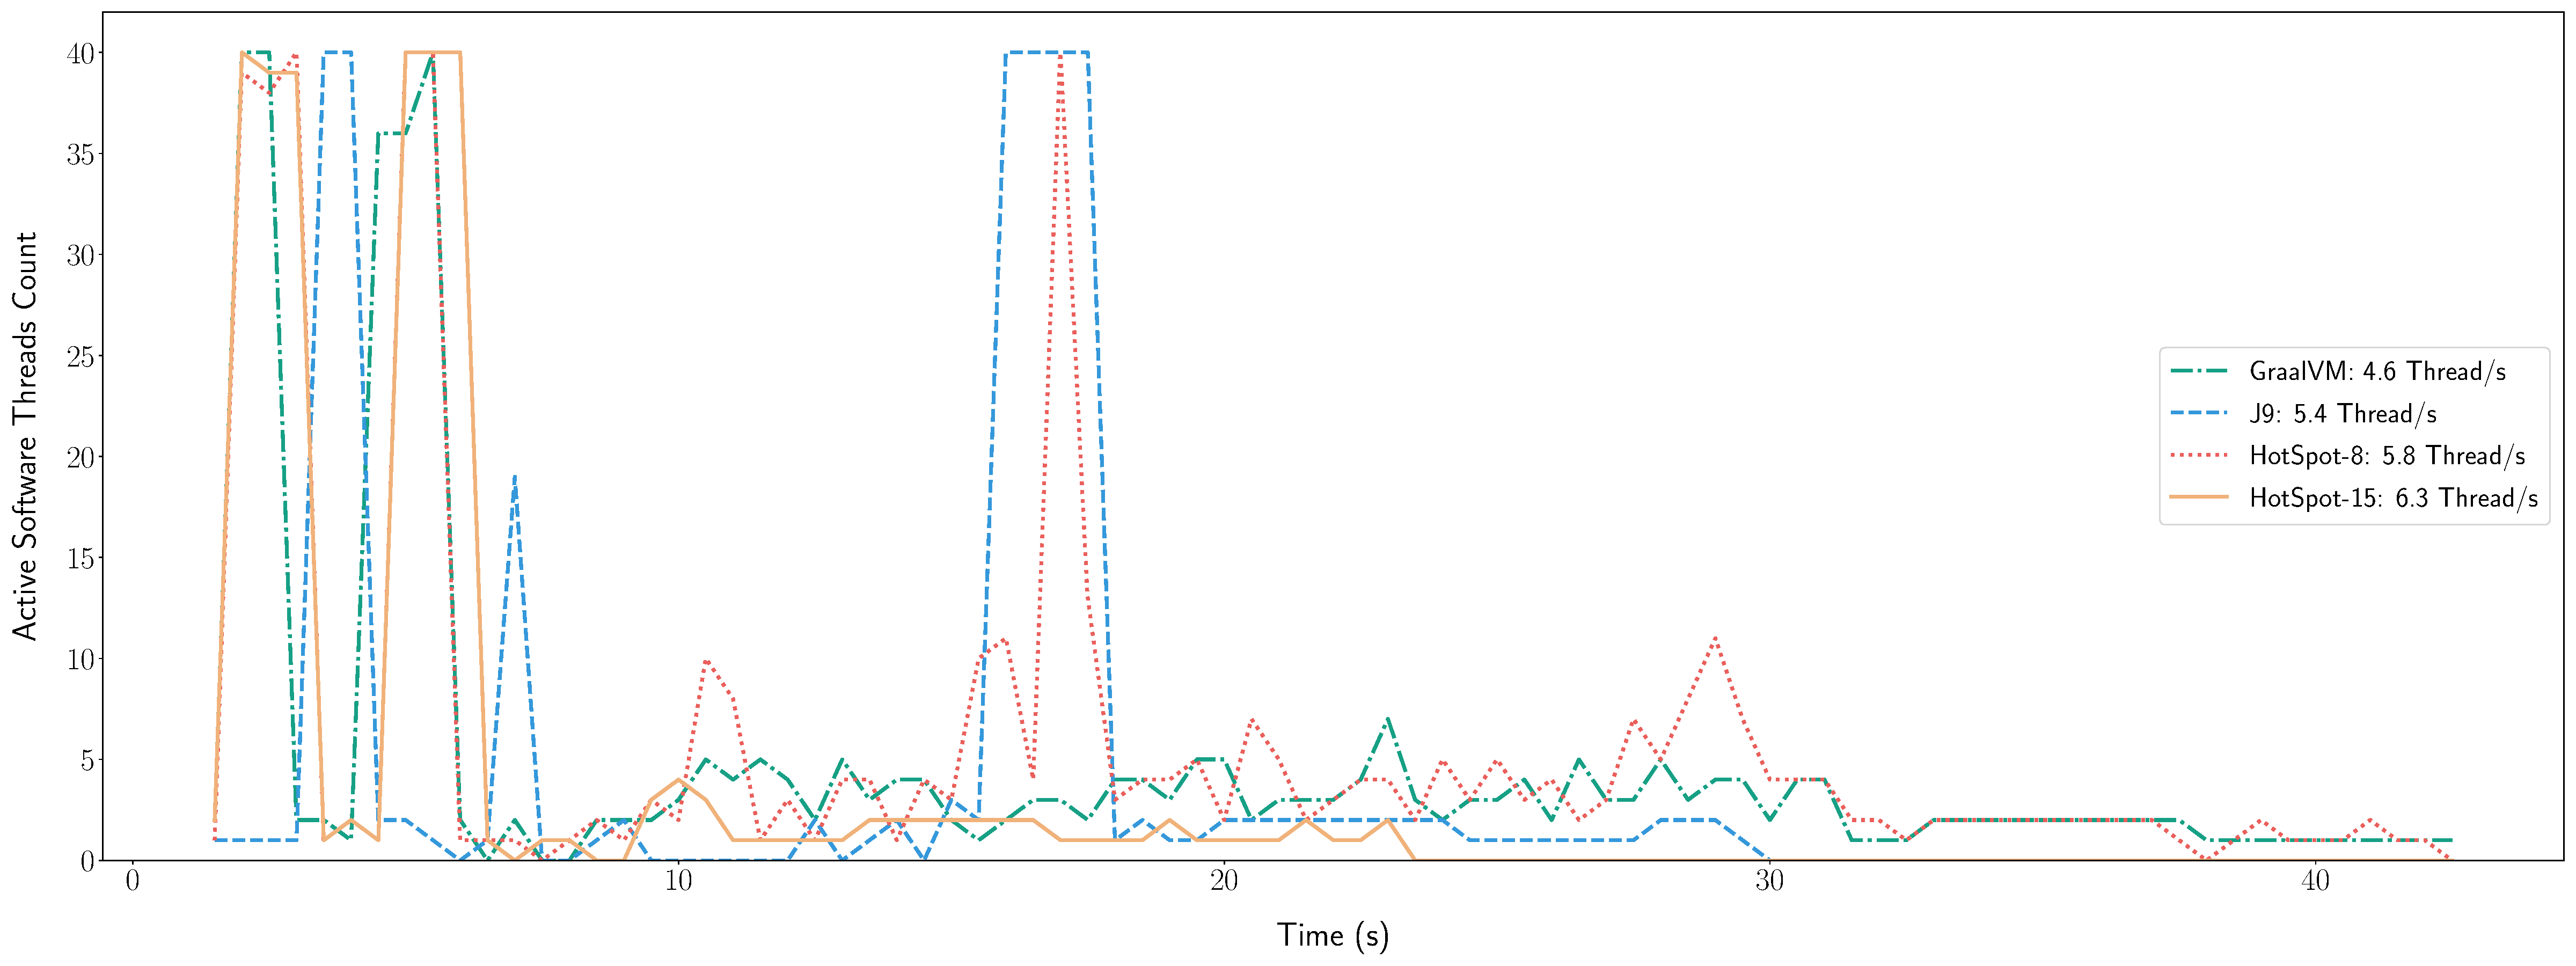
\includegraphics[width=.9\linewidth]{imgs/active_threads_reactors_chetemi_3}
        \centering
        \captionsetup{justification=centering}
        \caption{Active threads of \textsf{Reactors} when using \textsc{HotSpot}, \textsc{GraalVM}, or \textsc{J9}.}
        \label{fig:reactors_threads}
    \end{subfigure}
    %	\begin{subfigure}{\textwidth}
    %		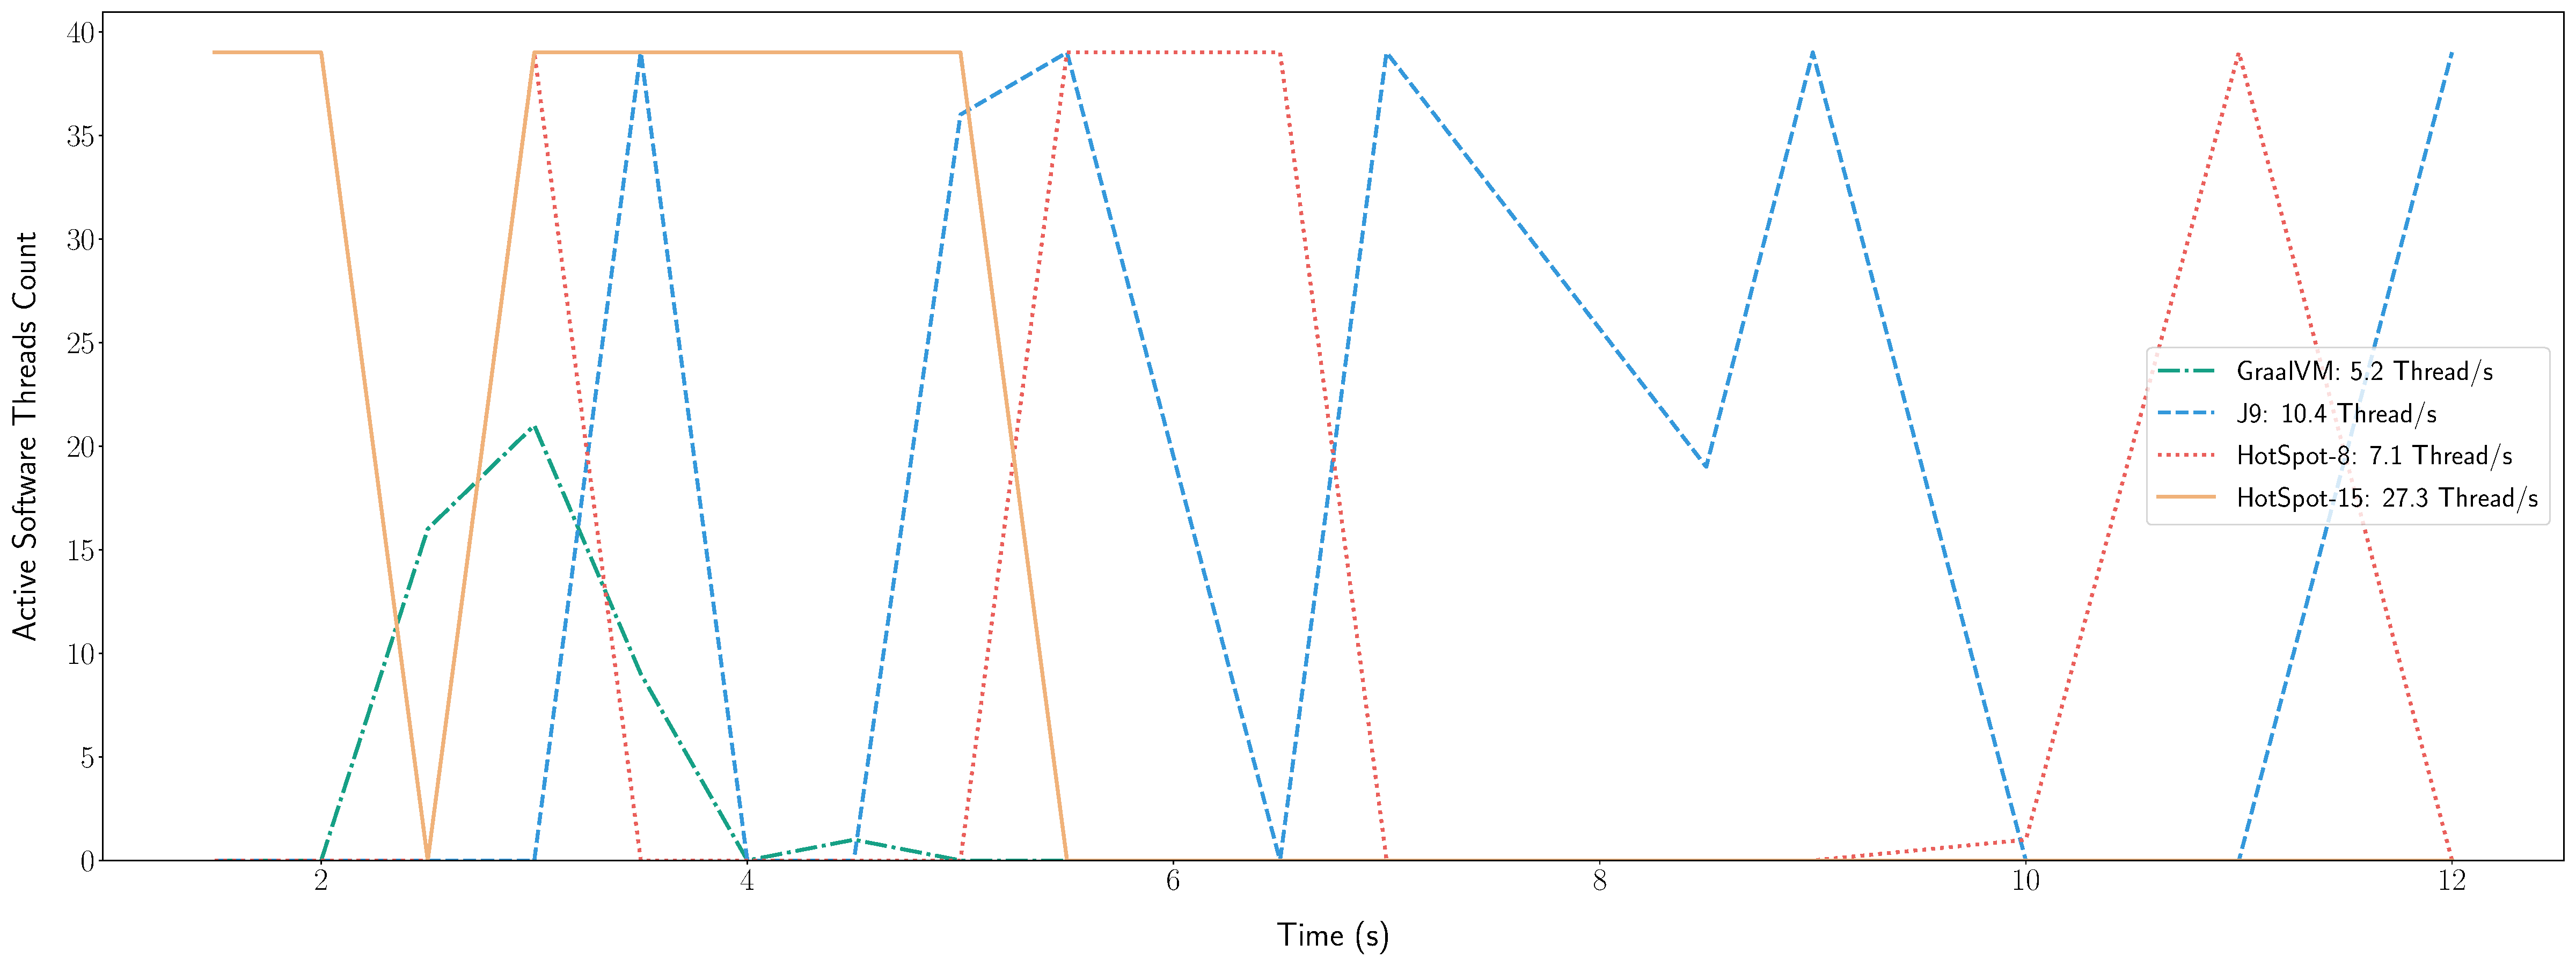
\includegraphics[width=.9\linewidth]{imgs/active_threads_scrabble_chetemi_3.pdf}
    %		\centering
    %		\captionsetup{justification=centering}
    %		\caption{Active threads of \textsf{Scrabble} when using \textsc{HotSpot}, \textsc{GraalVM}, or \textsc{J9}}
    %		\label{fig:scrabble_threads}
    %	\end{subfigure}
    \caption{Active threads evolution when using \textsc{HotSpot}, \textsc{GraalVM}, or \textsc{J9}.}
    \label{fig:threads}
\end{figure*}

\Cref{fig:threads} delivers a closer look to the thread allocation strategies adopted by JVM.
First, \Cref{fig:avrora_threads} illustrates the active threads count evolution over time (excluding the JVM-related threads, usually 1 or 2 extra threads depending on the execution phase) for \textsf{Avrora}.
One can notice through the figure that \textsc{J9} exploits the CPU more intensively by running much more parallel threads compared to other JVMs (an average of 5.1 threads per second for \textsc{J9} while the other JVMs do not exceed 1.5 thread per second).
Furthermore, the number of context switches is twice bigger for \textsc{J9}, while the number of soft page faults is twice smaller.
The efficient \textsc{J9} thread management explains why running the \textsf{Avrora} benchmark took much less time and consumed less energy, given that no other difference for the JIT or GC configuration was spotted between the JVMs.
Another key reason for the \textsc{J9}'s efficiency for the \textsf{Avrora} benchmark is memory allocation, as \textsf{OpenJ9} adopts a different policy for the heap allocation.
It creates a non-collectible \emph{thread local heap} (TLH) within the main heap for each active thread.
The benefit of cloning a dedicated TLH is the fast memory access for independent threads: each thread has its heap and no deadlock can occur.

The second example in \Cref{fig:reactors_threads} depicts the active threads evolution over time of the \textsf{Reactors} benchmark.
In this case, all the JVMs have a close average of threads per second.
Nevertheless, one can still observe that \textsc{HotSpot-15} and \textsc{J9} keep running faster, which confirms the results of \Cref{fig:all_benchs}, where both JVMs consume much less energy compared to \textsc{GraalVM} and \textsc{HotSpot-8}.
This difference in energy consumption between benchmarks can be less likely caused by thread management for the \textsf{Reactors} benchmark, as \textsc{HotSpot-8} reports on a higher average of active threads.
However, the TLH mechanism was not as efficient as for the \textsf{Avrora} benchmark, as dedicating a heap for each thread can also cause some extra memory usage for data duplication and synchronization, especially if a lot of data is shared between threads.

%In the case of the \textsf{Scrabble} benchmark illustrated in \Cref{fig:scrabble_threads}, one can see that \textsc{GraalVM} executed the benchmark much faster, and with even less threads.
%With only 5.2 threads/sec, \textsc{GraalVM} was able to be 50\% faster than \textsc{HotSpot-8} and \textsc{J9} and consuming the least energy, while the other JVMs ran more threads per second.
% This advocates that threads management was not the key factor here, thus requiring to further investigate other JVM settings. 
% \textsc{GraalVM} was faster and more energy efficient due to other JVM optimizations.

In conclusion, JVMs thread management can sometimes constitute a key factor that impacts software energy consumption.
However, we suggest checking and comparing JVMs before deploying a software, especially if the target application is parallel and multi-threaded.


\subsubsection{Just-in-Time Compilation}
The purpose of experiments on JIT is to highlight the different strategies that can impact software energy consumption within a JVM and between JVMs.
We identified a set of JIT compiler parameters for every JVM platform.

For \textsc{J9}, we considered fixing the intensity of the JIT compiler at multiple levels (\textsf{cold}, \textsf{warm}, \textsf{hot}, \textsf{veryhot}, and \textsf{scorching}).\footnote{\url{[https://www.eclipse.org/openj9/docs/jit/]}}
The hotter the JIT, the more code optimization to be triggered.
We also varied the minimum count method calls before a JIT compilation occurs (\textsf{10}, \textsf{50}, \textsf{100}), and the number of JIT instances threads (from \textsf{1} to \textsf{7}).
For \textsc{Hotspot-15}, we conducted experiments while disabling the tiered compilation (that generates compiled versions of methods that collect profiling information about themselves), and we also varied the JIT maximum compilation level from \textsf{0} to \textsf{4}, we also tried out \textsc{HotSpot} with a basic \textsc{GraalVM} JIT.
We note that level 0 of JIT compilation only uses the interpreter, with no real JIT compilation.
Levels 1, 2, and 3 use the C1 compiler (called client-side) with different amounts of extra tuning.
% Furthermore, the level 3 performs a full profiling.
The JIT C2 (also called server-side JIT) compiler only kicks in at level 4.

For \textsc{GraalVM}, we conducted experiments with and without the JVMCI (a Java-based JVM compiler interface enabling a compiler written in Java to be used by the JVM as a dynamic compiler).
We also considered both the community and economy configurations (no enterprise).
A JIT+AOT (\emph{Ahead Of Time}) disabling experiment has also been considered for all of the 3 JVM platforms.
\Cref{table:JIT} reports on the energy consumption of the experiments we conducted for most of the benchmarks and JIT configurations under study.

\begin{table*}
    \centering
    \caption{Energy consumption when tuning JIT settings on \textsc{HotSpot}, \textsc{GraalVM} \& J9}
    \label{table:JIT}
    \resizebox*{\linewidth}{!}{
        \begin{tabular}{cl|rr|rr|rr|rr|rr|rr|rr|rr|rr|rr}
            \toprule
            JVM & Mode         & \multicolumn{2}{c}{ALS} & \multicolumn{2}{c}{Avrora} & \multicolumn{2}{c}{Dotty} & \multicolumn{2}{c}{Fj-kmeans} & \multicolumn{2}{c}{H2} & \multicolumn{2}{c}{Neo4j} & \multicolumn{2}{c}{Pmd} & \multicolumn{2}{c}{Reactors} & \multicolumn{2}{c}{Scrabble} & \multicolumn{2}{c}{Sunflow}                                                                                                                                      \\
            \midrule
            \multirow{3}{*}{\sc GraalVM}
                & \em Default  & 2848                    & \em p-values               & 3861                      & \em p-values                  & 2271                   & \em p-values              & 948                     & \em p-values                 & 1959                         & \em p-values                & 3313       & \em p-values & 297       & \em p-values & 23452       & \em p-values & 452  & \em p-values & 335       & \em p-values \\
                & DisableJVMCI & 3099                    & \bf 0.001                  & 4012                      & \bf 0.041                     & 2694                   & \bf 0.001                 & \best 934               & \bf  0.011                   & \best 1771                   & \bf 0.005                   & 5086       & \bf  0.001   & 353       & \bf 0.001    & 25007       & \bf 0.007    & 503  & \bf 0.002    & 354       & 0.227        \\
                & Economy      & 4503                    & \bf 0.001                  & 3895                      & 0.793                         & 3466                   & \bf 0.001                 & 1306                    & \bf 0.002                    & 2560                         & \bf 0.001                   & 9525       & \bf  0.001   & \best 270 & \bf 0.001    & 30317       & \bf 0.001    & 649  & \bf 0.002    & 392       & \bf 0.002    \\
            \hline
            \multirow{12}{*}{J9}
                & \em Default  & 3792                    & \em p-values               & 2122                      & \em p-values                  & 3515                   & \em p-values              & 1271                    & \em p-values                 & 2426                         & \em p-values                & 4336       & \em p-values & 277       & \em p-values & 12705       & \em p-values & 734  & \em p-values & 476       & \em p-values \\
                & Thread 1     & 4157                    & \bf 0.001                  & 2121                      & 0.875                         & 4749                   & \bf 0.001                 & 1297                    & 0.097                        & 2597                         & 0.066                       & 4906       & \bf 0.001    & 350       & \bf 0.001    & 12800       & 0.713        & 948  & \bf 0.002    & 626       & \bf 0.005    \\
                & Thread 3     & 3849                    & 0.018                      & 2105                      & 0.713                         & 3574                   & 0.104                     & 1259                    & 0.371                        & 2450                         & 0.637                       & 4477       & \bf 0.005    & 294       & \bf 0.004    & 12647       & 0.875        & 795  & 0.021        & 457       & 0.27         \\
                & Thread 7     & 3843                    & 0.041                      & 2386                      & 0.372                         & 3511                   & 0.875                     & 1259                    & 0.25                         & 2424                         & 0.637                       & 4431       & 0.104        & 273       & 0.372        & 12600       & 0.875        & 808  & 0.055        & 463       & 0.372        \\
                & Count 0      & 8461                    & \bf 0.001                  & 2425                      & \bf 0.001                     & 4877                   & \bf 0.001                 & 2289                    & \bf 0.002                    & 3212                         & \bf 0.001                   & 10565      & \bf 0.001    & 744       & \bf 0.001    & 18084       & \bf 0.001    & 1476 & \bf 0.002    & 922       & \bf 0.001    \\
                & Count 1      & 4281                    & \bf 0.001                  & 2150                      & 0.431                         & 3164                   & \bf 0.001                 & 1841                    & \bf 0.002                    & 2546                         & 0.431                       & 7166       & \bf 0.001    & 272       & 0.128        & 14715       & \bf 0.001    & 1005 & \bf 0.002    & 514       & 0.052        \\
                & Count 10     & 3980                    & \bf 0.001                  & 2431                      & 0.713                         & 3771                   & \bf 0.001                 & 1312                    & \bf 0.011                    & 2779                         & \bf  0.003                  & 4979       & \bf 0.001    & 299       & \bf 0.001    & 12000       & 0.104        & 860  & \bf 0.005    & 1182      & \bf 0.001    \\
                & Count 100    & 3878                    & \bf 0.007                  & 2141                      & 0.713                         & 3469                   & 0.227                     & 1363                    & 0.523                        & 2513                         & 0.128                       & 4547       & \bf 0.001    & 262       & 0.031        & 12313       & 0.024        & 768  & 0.16         & 634       & \bf 0.004    \\
                & Cold         & 6788                    & \bf 0.001                  & 2134                      & 0.637                         & 4855                   & \bf 0.001                 & 1636                    & \bf 0.002                    & 2873                         & \bf  0.001                  & 7250       & \bf 0.001    & 275       & 0.372        & 20380       & \bf 0.001    & 870  & \bf 0.005    & 386       & \bf 0.001    \\
                & Warm         & 4594                    & \bf 0.001                  & 2112                      & 0.713                         & 4253                   & \bf 0.001                 & 1244                    & 0.055                        & 2521                         & 0.128                       & 5305       & \bf 0.001    & 411       & \bf 0.001    & 13726       & \bf 0.001    & 913  & \bf 0.002    & 336       & \bf 0.001    \\
                & Hot          & 7553                    & \bf 0.001                  & 2310                      & \bf 0.001                     & 12749                  & \bf 0.001                 & 1452                    & \bf 0.002                    & 3973                         & \bf 0.001                   & 8979       & \bf 0.001    & 857       & \bf 0.001    & 36534       & \bf 0.001    & 1180 & \bf 0.002    & 506       & 0.128        \\
                & VeryHot      & 15113                   & \bf 0.001                  & 3300                      & \bf 0.001                     & 18235                  & \bf 0.001                 & 2430                    & \bf 0.002                    & 7205                         & \bf 0.001                   & 19359      & \bf 0.001    & 793       & \bf 0.001    & 38303       & \bf 0.001    & 5420 & \bf 0.002    & 1692      & \bf 0.001    \\
                & Schorching   & 18316                   & \bf 0.001                  & 3541                      & \bf 0.001                     & 21686                  & \bf 0.001                 & 2514                    & \bf 0.002                    & 7855                         & \bf 0.001                   & 26409      & \bf 0.014    & 808       & \bf 0.001    & 43929       & \bf 0.001    & 5583 & \bf 0.002    & 1778      & \bf 0.001    \\
            \hline
            \multirow{5}{*}{\sc HotSpot}
                & \em Default  & 2997                    & \em p-values               & 4014                      & \em p-values                  & 2516                   & \em p-values              & 934                     & \em p-values                 & 1796                         & \em p-values                & 4787       & \em p-values & 323       & \em p-values & 11685       & \em p-values & 530  & \em p-values & 325       & \em p-values \\
                & Graal        & 2999                    & 0.637                      & 3971                      & 0.318                         & 2512                   & 0.318                     & 929                     & 0.609                        & \best 1662                   & \bf 0.007                   & 4750       & 0.372        & 327       & 0.189        & 11548       & 0.523        & 537  & 0.701        & 338       & 0.564        \\
                & Lvl 0        & 491443                  & /                          & 14484                     & /                             & 84395                  & /                         & /                       & /                            & 52344                        & /                           & 356287     & /            & 1073      & /            & 148381      & /            & /    & /            & 14559     & /            \\
                & Lvl 1        & /                       & /                          & \best 3731                & \bf 0.001                     &  3302             & \bf 0.001                 & 1256                    & \bf 0.002                    & 2523                         & \bf 0.001                   & 8304       & \bf 0.001    & \best 222 & \bf 0.001    & 22410       & \bf 0.002    & 735  & \bf 0.002    & \best 277 & \bf 0.007    \\
                & Lvl 2        & 3079                    & \bf 0.004                  & 4110                      & 0.189                         & 3723                   & \bf 0.001                 & 22547                   & \bf 0.002                    & 2840                         & \bf 0.001                   & 19058      & \bf 0.001    & 226       & \bf 0.001    & 40701       & \bf 0.002    & 2291 & \bf 0.002    & 4131      & \bf 0.001    \\
                & Lvl 3        & 16375                   & \bf 0.001                  & 7729                      & \bf 0.001                     & 6789                   & \bf 0.001                 & 144914                  & \bf 0.002                    & 4139                         & \bf 0.001                   & 44594      & \bf 0.001    & 330       & \bf 0.005    & 190124      & \bf 0.002    & 9070 & \bf 0.002    & 10449     & \bf 0.001    \\
                %& Lvl 4        & \best 2977              & 0.066                      & 3964                      & 0.27                          & 2509                   & 0.958                     & 932                     & 1.0                          & \best 1692                   & \bf 0.004                   & 4766       & 0.713        & 334       & 0.27         & 11614       & 0.798        & 528  & 1.0          & 332       & 0.637        \\
                & NotTired     & 3254                    & \bf 0.001                  & 3901                      & 0.189                         &  3110             & \bf 0.001                 & \best 912               & \bf 0.021                    & 1846                         & 0.227                       & \best 3844 & \bf 0.001    & 933       & \bf  0.001   & \best 11256 & \bf 0.041    & 588  & \bf 0.003    & 405       & \bf 0.001    \\

            \bottomrule
        \end{tabular}
    }
\end{table*}

The $p$-values are computed with the Mann-Whitney test, with a null hypothesis of the energy consumption being equal to the default configuration.
The $p$-values in bold show the values that are significantly different from the default configuration with a 95\% confidence, where the values in green highlight the strategies that consumed significantly less energy than the default (less energy and significant $p$-value).


%The results show that none of the 3 JVMs has the best or worst performance for all benchmarks.

For \textsc{J9}, we noticed that adopting the default JIT configuration is always better than specifying a custom JIT intensity.
The \textsf{warm} configuration delivers the closest results to the best results observed with the default configuration.
Moreover, choosing a low minimum count of method calls seems to have a negative effect on the execution time and energy consumption.
The only parameter that can give better performance than the default configuration in some cases is the number of parallel JIT threads---using 3 and 7 parallel threads---but is not statistically significant.

For \textsc{GraalVM}, the default community configuration is often the one that consumes the least energy.
Disabling the JVMCI can---in some cases---have a benefit (16\% of energy consumption reduction for the \textsf{H2} benchmark), but still gave overall worst results (80\% more energy consumption for the \textsf{Neo4J} benchmark).
In addition, switching the economy version of the \textsc{GraalVM} JIT often results in consuming more energy and delaying the execution.

For \textsc{HotSpot}, keeping the default configuration of the JIT is also mostly good.
The usage of the C2 JIT is often beneficial (JIT level 4) in most cases while using the \textsc{GraalVM} JIT reported similar energy efficiency.
Yet, some benchmarks showed that using only the C1 JIT (JIT level 1) is more efficient and even outperforms the usage of the C2 compiler.
10\% on \textsf{Avrora} and 30\% on \textsf{Pmd} are examples of energy savings observed by using the C1 compiler.
However, being limited to the C1 compiler can also cause a huge degradation in energy consumption, such as 32\% and 34\% of additional energy consumed for the \textsf{Dotty} and \textsf{FJ-kmeans} benchmarks, respectively.
Hence, if it is a matter of not using the C2 JIT, the experiments have shown that the level 1 JIT is always the best, compared to levels 2 or 3 that also use the C1 JIT, but with more options, such as code profiling that impacts negatively the performance and the energy efficiency.
Level 0 JIT compilation should never be an option to consider.
No $p$-value has been computed for Level 0, due to the limited amount of iterations executed with this mode (very high execution time, clearly much more consumed energy).

Globally, we conclude through these experiments that keeping the default JIT configuration was more energy efficient in ~80\% of our experiments and for the 3 classes of JVMs.
This advocates using the default JIT configuration that can often deliver near-optimal energy efficiency.
Although, some other configurations, such as using only the C1 JIT or disabling the JVMCI could be advantageous in some cases.


\subsubsection{Garbage Collection}
Changing or tuning the GC strategy has been acknowledged to impact the JVM performances~\cite{10.1145/2568088.2568097}.
To investigate if this impact also benefits energy consumption, we conducted a set of experiments on the selected JVMs.
We considered different garbage collector strategies with a limited memory quantity of 2\,GB, and recorded the execution time and the energy consumption.
The tested GC strategies options mainly vary between \textsc{J9} and the other 2 JVMs, as detailed in \Cref{table:GCJ9}.

\begin{table}
    \centering
    \caption{The different \textsc{J9} GC policies}
    \label{table:GCJ9}
    \small
    \begin{tabular}{|p{0.2\columnwidth}|p{0.7\columnwidth}|}
        \hline
        \textbf{Policy}              & \textbf{Description}                                                                                                         \\
        \hline
        \hline
        \textsf{Balanced}            & Evens out pause times \& reduces the overhead of the costlier operations associated with GC                                  \\
        \hline
        \textsf{Metronome}           & GC occurs in small interruptible steps to avoid stop-the-world pauses                                                        \\
        \hline
        \textsf{Nogc}                & Handles only memory allocation \& heap expansion, with no memory reclaim                                                     \\
        \hline
        \textsf{Gencon}\,(default)   & Minimizes GC pause times without compromising throughput, best for short-lived objects                                       \\
        \hline
        \textsf{Concurrent Scavenge} & Minimizes the time spent in stop-the-world pauses by collecting nursery garbage in parallel with running application threads \\
        \hline
        \textsf{optthruput}          & Optimized for throughput, stopping applications for long pauses while GC takes place                                         \\
        \hline
        \textsf{Optavgpause}         & Sacrifices performance throughput to reduce pause times compared to \textsf{optthruput}                                      \\
        \hline
    \end{tabular}
\end{table}

For \textsc{HotSpot} and \textsc{GraalVM}, we also considered many GC policies, as described in \Cref{table:GCHS}.
Furthermore, other GC settings have also been tested for all JVM platforms, such as the \emph{pause time}, the \emph{number of parallel threads} and \emph{concurrent threads} and \emph{tenure age}.

\begin{table}
    \centering
    \caption{The different \textsc{HotSpot}/\textsc{GraalVM} GC policies}
    \label{table:GCHS}
    \small
    \begin{tabular}{|p{0.2\columnwidth}|p{0.7\columnwidth}|}
        \hline
        \textbf{Policy}          & \textbf{Description}                                                                                                                 \\
        \hline
        \hline
        \textsf{G1GC}\,(default) & Uses concurrent \& parallel phases to achieve low-pauses GC and maintain good throughput                                             \\
        \hline
        \textsf{SerialGC}        & Uses a single thread to perform all garbage collection work (no threads communication overhead)                                      \\
        \hline
        \textsf{ParallelGC}      & Known as throughput collector: similar to \textsf{SerialGC}, but uses multiple threads to speed up garbage collections for scavenges \\
        \hline
        \textsf{parallelOldGC}   & Use parallel garbage collection for the full collections, enabling it automatically enables the \textsf{ParallelGC}                  \\
        \hline
    \end{tabular}
\end{table}

\begin{table*}
	\centering
	\caption{Energy consumption when tuning GC settings on \textsc{HotSpot}, \textsc{GraalVM} \& J9}
	\label{table:GC}
	\resizebox*{\linewidth}{!}{
		\begin{tabular}{cl|rr|rr|rr|rr|rr|rr|rr|rr|rr}
			\toprule
			% JRE & Mode &  Als & &  Avrora & &  Dotty & &   H2 & &  Lusearch & &  Neo4j & &  Pmd & &  RePactors & &  Scrabble & &  Sunflow & \\
			JVM & Mode                & \multicolumn{2}{c}{ALS} & \multicolumn{2}{c}{Avrora} & \multicolumn{2}{c}{Dotty} & \multicolumn{2}{c}{H2} & \multicolumn{2}{c}{Neo4j} & \multicolumn{2}{c}{Pmd} & \multicolumn{2}{c}{Reactors} & \multicolumn{2}{c}{Scrabble} & \multicolumn{2}{c}{Sunflow}                                                                                                                               \\
			\midrule
			\multirow{9}{*}{\sc GraalVM}
			    & \em Default         & 2570                    & \em  p-values              & 4153                      & \em p-values           & 2223                      & \em p-values            & 1870                         & \em p-values                 & 5256                        & \em p-values & 281       & \em p-values & 2611       & \em p-values & 410        & \em p-values & 353        & \em p-values \\
			    & 1Concurent          & 2567                    & 0.403                      & \best4007                      & \bf 0.023              & 2220                      & 1.000                   & 1883                         & 0.982                        & 5368                        & 1.000        & 286       & 0.182        & 2664       & 1.000        & 413        & 0.885        & 347        & 0.573        \\
			    & 1Parallel           & 2668                    & \bf 0.012                  & \best 3904                &  \bf 0.008            & 2228                      & 0.835                   & 2022                         & \bf 0.000                    & 5836                        & \bf 0.012    & 298       & \bf 0.000    & 2869       & 0.144        & 561        & \bf 0.030    & \best 317  &  \bf0.000  \\
			    & 5Concurent          & 2570                    & 0.676                      & 4117                      & 0.161                  & 2215                      & 0.210                   & 1862                         & 0.505                        & 5259                        & 1.000        & 282       & 0.980        & 2611       & 0.531        & 414        & 0.885        & 362        & 0.356        \\
			    & 5Parallel           & 2561                    & 0.676                      & \best3863                      & \bf 0.012              & 2237                      & 1.000                   & 1910                         & 0.103                        & 5223                        & 0.403        & 282       & 0.538        & 2682       & 0.531        & 424        & 0.112        & 353        & 0.758        \\
			    & DisableExplicitGC   & 2559                    & 0.210                      & \best3911                      & \bf 0.003              & 2215                      & 1.000                   & 1978                         & \bf 0.018                        & 5106                        & 0.210        & 281       & 0.758        & 2704       & 0.676        & 400        & 0.312        & \best332        & \bf 0.036    \\
			    & ParallelCG          & 2720                    & \bf 0.012                  & 4016                      & 0.206                  & 2237                      & 0.531                   & 1945                         & \bf 0.000                    & 13172                       & \bf 0.037    & 282       & 0.878        & \best 2267 &  \bf 0.022  & 545        & \bf 0.030    & \best329        & \bf 0.003    \\
			    & ParallelOldGC       & 2715                    & \bf 0.012                  & 4032                      & 0.103                  & 2221                      & 1.000                   & 1925                         & \bf 0.002                    & 13362                       & /            & 282       & 0.918        & \best 2514       & \bf 0.012    & 535        & \bf 0.030    & \best 329        & \bf 0.008    \\
			%	& G1                &\best 2557 &      &    4080 &    0.124  &      2221 & 1.000   &    1887 & 0.408 &      192 &0.218 &       5393 &1.000 &    284 &0.383 &    2600 &0.403 &      415 &0.885 &      363 &0.330 \\

			\hline
			\multirow{9}{*}{J9}
			    & \em Default         & 3371                    & \em p-values               & 2243                      & \em p-values           & 3237                      & \em p-values            & 2107                         & \em p-values                 & 6277                        & \em p-values & 232       & \em p-values & 1644       & \em p-values & 589        & \em p-values & 510        & \em p-values \\
			    & Balanced            & 9012                    & \bf 0.012                  & 2232                      & 0.597                  & 3429                      & \bf 0.012               & 2247                         & \bf 0.002                    & 8853                        & \bf 0.012    & 235       & 0.412        & 1902       & \bf 0.020    & 661        & 0.061        & 519        & 0.505        \\
			    & ConcurrentScavenge  & 3487                    & \bf 0.012                  & 2270                      & 0.280                  & 3388                      & \bf 0.012               & 2319                         & \bf 0.001                    & 6857                        & \bf 0.012    & 233       & 0.878        & 1705       & 0.903        & 639        & 0.194        & 546        & \bf 0.018    \\
			    & Metronome           & \best 2098              & \bf 0.012                & 2265                      & 0.505                  & 3815                      & \bf 0.012               & 2717                         & \bf 0.000                    & 12103                       & \bf 0.012    & 239       & \bf 0.022    & 2089       & \bf 0.020    & 758        & \bf 0.030    & \best 422  & \bf 0.000  \\
			    & Nogc                & 3454                    & \bf 0.022                  & 2239                      & 0.872                  & 3259                      & 0.144                   & 2207                         & 0.031                        & 61781                       & \bf 0.012    & 227       & 0.151        & \best 1505 & \bf 0.066  & 711        & \bf 0.030    & 499        & 0.720        \\
			    & Optavgpause         & 3601                    & \bf 0.012                  & 2431                      & 0.370                  & 3425                      & \bf 0.012               & 2169                         & 0.297                        & 7495                        & \bf 0.012    & 253       & \bf 0.000    & 1772       & 0.391        & 1089       & \bf 0.030    & 478        & \bf 0.046    \\
			    & Optthruput          & 3357                    & 1.000                      & 2432                      & 0.241                  & 3178                      & 0.403                   & 2194                         & 0.139                        & 6324                        & 0.835        & 232       & 0.878        & 1554       & 0.111        & 640        & 0.194        & \best 429        & \bf 0.000    \\
			    & ScvNoAdaptiveTenure & 3494                    & \bf 0.012                  & 2253                      & 0.800                  & 3248                      & 0.835                   & 2161                         & 0.103                        & 8442                        & \bf 0.012    & 228       & 0.137        & 1908       & \bf0.020     & 618        & 0.665        & 528        & 0.218        \\
			%	& Gencon              &      3387 &        &      2436 &        &    3234 &        &\best 2079 &      &    200 & &     6313 & &      232 &        &      1642 &        &     596 & &    524 & \\

			\hline
			\multirow{11}{*}{\sc HotSpot}
			    & \em Default         & 2765                    & \em p-values               & 4115                      & \em p-values           & 2492                      & \em p-values            & 1673                         & \em p-values                 & 8152                        & \em p-values & 316       & \em p-values & 1546       & \em p-values & 484        & \em p-values & 347        & \em p-values \\
			    & 1Concurent          & 2775                    &  0.060                  & 4137                      & 0.346                  & 2493                      & 0.676                   & 1675                         & 0.918                        & 8062                        & 0.531        & 316       & 0.383        & 1533       & 0.665        & 478        & 0.470        & 334        & \bf 0.218    \\
			    & 1Parallel           & 2863                    & \bf 0.012                  & 4142                      & 0.800                  & 2526                      & \bf 0.037               & 1853                         & \bf 0.001                    & 8270                        & 0.676        & 334       & \bf 0.000    & 1747       & \bf 0.030    & 592        & \bf 0.030    & \best  320 & \bf 0.002  \\
			    & 5Concurent          & 2758                    & 0.676                      & 4091                      & 0.872                  & 2485                      & 0.296                   & 1681                         & 0.608                        & 8087                        & 0.835        & 314       & 0.330        & 1497       & 0.665        & \best  469 & \bf 0.030  & 336        & 0.259        \\
			    & 5Parallel           & 2767                    & 0.144                      & 4176                      & 0.077                  & 2473                      & 0.060                   & 1654                         & 0.720                        & 8046                        & 0.835        & 316       & 0.573        & 1546       & 0.470        & 489        & 0.470        & 342        & 0.573        \\
			    & DisableExplicitGC   & \best 2734                    & \bf 0.012                  & 4062                      & 0.448                  & 2483                      & 0.835                   & 1702                         & 0.248                        & \best 7710                        & \bf 0.037    & 312       & 0.200        & 1545       & 0.470        & 470        & 0.061        & \best 325        & \bf 0.014    \\
			    & ParallelCG          & \best 2653                    & \bf 0.012                  & 4064                      & 0.629                  & \best  2356               & \bf 0.012             & \best 1602                   & \bf 0.008                  & 8953                        & 0.060        & \best 300 & \bf 0.000  & 1476       & 0.885        & 579        & \bf 0.030    & 336        & 0.081        \\
			    & ParallelOldGC       & 2764                    & 0.531                      & 4070                      & 0.872                  & 2525                      & 0.802                   & 1675                         & 0.959                        & 7963                        & 0.403        & 314       & 0.720        & 1582       & 0.194        & 475        & 0.470        & 333        & 0.151        \\
			    & SerialGC            & \best 2593              & \bf 0.012                & 4083                      & 0.395                  & \best 2378                      & \bf 0.012               & \best 1620                         & \bf 0.046                    & \best 5745                  & \bf 0.012  & \best 307       & \bf 0.002    & 1672       & 0.061        & 601        & \bf 0.030    & 352        & 0.473        \\
			%	& G1                &    2768 &        &    4066 &        &     2498 &        &      1715 &        &     239 &        &    8131 &        &    314 &        &    1546 &        &     469 &        &     337 & \\

			%	& Epsilon           & 3005 &        &   8342 &        & 7084 &        &5063 &        &     4260 &        & 14427 &        &    4400 &        & 2105 &        & 4980 &        & 4594 & \\
			\bottomrule
		\end{tabular}
	}
\end{table*}

\Cref{table:GC} summarizes the results of all the tested GC strategies with our selected benchmarks and the $p$-values of the Mann-Whitney test, with a null hypothesis of the energy consumption being equal to the default configuration with a 95\% confidence.
The $p$-values in bold show the values that are significantly different from the default configuration, whereas the values in green highlight the strategies that consumed significantly less energy than the default.
For \textsc{GraalVM}, one can see that the GC default configuration is efficient in most experiments, compared to other strategies.
The main noticeable impact is related to the \textsf{ParallelGC} and \textsf{ParallelOldGC}.
In fact, the \textsf{ParallelGC} can be 13\% more energy efficient in some applications with a significant $p$-value, such as \textsf{Reactors}, compared to default.
However, the same GC strategy can cause the software to consume twice times more, as for the \textsf{Neo4j} benchmark, due to the high communications between the GC threads, and the fragmentation of the memory.

For \textsc{J9}, the default \textsf{Gencon} GC causes the software to report an overall good energy efficiency among the tested benchmarks.
However, other GC can cause better or worse energy consumption than \textsf{Gencon} depending on workloads.
Using the \textsf{Metronome} GC consumes ~35\% less energy for the \textsf{ALS} benchmark and ~17\% less energy for the \textsf{Sunflow} benchmark, but it also consumes 100\% more energy for the \textsf{Neo4j} benchmark and 28\% more energy for \textsf{Reactors}.
The reason is that \textsf{Metronome} occurs in small preemptible steps to reduce the GC cycles composed of many GC quanta.
This suits well for real-time applications and can be very beneficial when long GC pauses are not desired, as observed for \textsf{ALS}.
However, if the heap space is insufficient after a GC cycle, another cycle will be triggered with the same ID.
As \textsf{Metronome} supports class unloading in the standard way, there might be pause time outliers during GC activities, inducing a negative impact on the \textsf{Neo4j} execution time and energy consumption.

The same goes for the \textsf{Balanced} GC that tries to reduce the maximum pause time on the heap by dividing it into individually managed regions.
The \textsf{Balanced} strategy is preferred to reduce the pause times that are caused by global GC, but can also be disadvantageous due to the separate management of the heap regions, such as for \textsf{ALS} where it consumed about three times the energy consumption, compared to the default \textsf{Gencon} GC.
On the other hand, the \textsf{Optthruput} GC, which stops the application longer and less frequently, gave very good overall results and sometimes even outperformed the \textsf{Gencon} GC by a small margin.
Other JVM parameters, such as the \textsf{ConcurrentScavenge} or \textsf{noAdaptiveTenure} did not have a substantial impact during our experiments.

Finally, the results of \textsc{HotSpot} shared similarities with \textsc{GraalVM}.
The \textsf{ParallelGC} happened to give better (6\% for \textsf{Dotty}) or worst (10\% for \textsf{Neo4j}) energy efficiency compared to the default GC.
On the other hand, \textsf{ParallelOldGC} and \textsf{Serial} GC gave better results than the default G1 GC.
More specifically, the second one consumed 30\% and 6\% less energy than the default GC for the \textsf{Neo4j} and \textsf{Dotty} benchmarks, respectively.
%Moreover, the Epsilon GC gave worst results compared to the default GC, and also used much more memory( 63 Gb for Epsilon GC against 4Gb for default GC).
%It even stopped working for many benchmarks due to the heap memory being saturated.
The most interesting result for \textsc{HotSpot} is the 30\% energy reduction obtained with the \textsf{Serial} GC.
This last was also more efficient on ALS (6\% less energy), compared to the default G1 GC, due to its single-threaded GC that only uses one CPU core.
%Moreover, it's single threaded GC that uses one CPU core gave it the edge by quite a decent margin of 30\% on the h2 benchmark.
%Disabling the explicit GC also trends to give better results than the default GC configurations. Same as for GraalVM, using the concurrent configuration of the default GC is often better than the parallel one or default one (up to 50\% for neo4j benchmark).

Unfortunately, we cannot convey predictive patterns on how to configure the GC to optimize energy efficiency.
However, some considerations should be taken into account when choosing the GC, such as the garbage collection time, the throughput, etc.
Other settings are less trivial to determine, such as tenure age, memory size, and GC threads count.
Experiments should thus be conducted on the software to tune the most convenient GC configuration to achieve better energy efficiency in production.

Therefore, we noticed during our experiments that, even if using the default GC configuration ensures an overall steady and correct energy consumption, we still found other settings that reduce that energy consumption in ~50\% of our experiments.
Tuning the GC according to the hosted app/benchmark is thus critical to reducing energy consumption.

\bigbreak
\begin{mdframed}[]
    To answer \textbf{RQ\,2}, we conclude that users should be careful while choosing and configuring the garbage collector as substantial energy enhancements can be recorded from one configuration to another.
    The default GC consumes more energy than other strategies in most situations.
    % choosing the most convenient GC strategy in thus very important to achieve a better software energy efficiency. 
    However, keeping the default JIT parameters often delivers near-optimal energy efficiency.
    In addition, the JVM platforms can handle differently multi-threaded applications and thus consume a different amount of time/energy.
    Dedicated performance tuning evaluations should therefore be conducted on such software to identify the most energy-efficient platform and settings.
\end{mdframed}


\section{Threats to Validity}\label{sec:threats}
Several issues may affect the validity of our work.
First, we have the use of the Intel\,RAPL, one of the most accurate available tools to measure the energy consumption of software~\cite{Khan:2018:RAE:3199681.3177754,10.1145/2989081.2989088}.
However, RAPL only gives the global energy consumption and no fine-grained measures at process or thread levels.
We used bare-metal hardware with a minimal OS and turned off all the non-essential services and daemons to limit the overhead that the OS may add to the execution, even if it is not substantial~\cite{opaper}.

Another measurement issue is the CPU energy variation within machines (cf. \Cref{chapter:benchmarking}), thus we executed all the comparable tests on the same node and with the recommended settings to mitigate this threat.

Benchmarks' execution time could also constitute a more subtle threat to the validity of our work, especially for some benchmarks that run fast, such as the \textsf{Pmd} benchmark.
We thus gave a lot of attention to how long the benchmark is running for the hardware we used, and we tuned the input data workloads to execute benchmarks for at least many (from 10 to hundreds) seconds.
Experiments ran at least 30 times to compute the average consumption and the associated standard deviation, therefore reasoning over reasonable dispersion around the average.

How generalizable are our results?
We believe that our study conclusions and guideline remain empirical, as we do not intend to generalize any result we obtained for some JVM or benchmark.
We provide practitioners with some prerequisites to check before software deployment to reduce the software energy footprint by considering the JVM and its settings.


\section{Tools and contributions}
\textsf{J-Referral} is an open-source tool designed to assist developers and practitioners in selecting the most energy-efficient JVM configuration for their software..
\Cref{table:j-referral} illustrates an example of the final report returned by \textsf{J-Referral}.
The tool was tested for 2 Java projects: \textsf{Zip4J}\footnote{\url{https://github.com/srikanth-lingala/zip4j}} and \textsf{K-nucleotide}.\footnote{\url{https://benchmarksgame-team.pages.debian.net/benchmarksgame/performance/knucleotide.html}}
\textsf{Zip4J} runs a large file compression, while \textsf{K-nucleotide} extracts a DNA sequence, and updates a hashtable of k-nucleotide keys to count specific values.
The short report presented in \Cref{table:j-referral} shows the ratio of potential energy saving between the most and least energy consuming tested JVM (40\% and 70\% energy savings for \textsf{Zip4J} and \textsf{K-nucleotide}, respectively).
Options are available for \textsf{J-Referral} to obtain much more detailed reports including execution time, DRAM usage, split DRAM vs. CPU consumption, etc.
The tool is available as \emph{open-source software} (OSS) from our GitHub repository.\footnote{\url{https://github.com/chakib-belgaid/jreferral}}

\begin{table}
    \centering
    \caption{\textsf{J-Referral} recommendations.}
    \label{table:j-referral}
    \small
    \begin{tabular}{|c|c|c|c|c|}
        \hline
        \textbf{Project}                 & \textbf{Metric} & \textbf{Energy} & \textbf{JVM}       & \textbf{Execution flags} \\
        \hline
        \multirow{2}{*}{\textsf{Zip4J}}  & Least energy    & \best 2210\,J   & \best 16-sapmchn   & \best default            \\
        \cline{2-5}
                                         & Most energy     & 3680\,J         & 8.0.292-J9         & default                  \\
        \hline
        \hline
        \multirow{2}{*}{\textsf{K-nucl}} & Least energy    & \best 1296\,J   & \best 21.1.r16-grl & \best default            \\
        \cline{2-5}
                                         & Most energy     & 4433\,J         & 15.0.1-J9          & -Xjit:optlevel=cold      \\
        \hline
    \end{tabular}
\end{table}

\clearpage
\section{Summary}

This chapter describes an empirical investigation of contrast in energy consumption that some of the most well-known and widely supported JVM platforms can exhibit as well as the important factors that can influence this energy consumption.
During our experiments, we investigated 12 well-known and diverse-purpose Java benchmarks, as well as 52 JVMs, including many versions of 11 different distributions. 
Our findings revealed that various JVMs share energy efficiency and may be classified into three major classes: \textsc{HotSpot}, \textsc{J9}, and \textsc{GraalVM}.
However, the three JVM classes can show substantially different energy efficiency depending on the workloads and/or application.
While there was no clear champion in terms of energy consumption,\textsc{GraalVM} recorded the highest energy efficiency for the most of benchmarks. Nevertheless, depending on the workload, each JVM can achieve higher or worse efficiency.
One explanation could be thread management policy, as seen with \textsc{J9} when running \textsf{Avrora}.

Additionally, numerous JVM settings can cause changes in energy consumption. Our experiments revealed that the JVM's default JIT compiler is frequently near-optimal in at least 80\% of the experiments. 

On the other hand , the default GC outperformed the other strategies in just half of our experiments, with some significant benefits reported when employing different GCs based on the application characteristics. Our primary observations and recommendations can be stated as follows:
\begin{inparaenum}[\em i)]
    \item testing software on the 3 classes of JVM and identifying the one that consumes the least is a good practice, especially for multi-threading purposes,
    \item while the JVM default JIT give often good energy consumption results, some settings may improve the energy consumption and could be tested,
    \item the choice of the GC may lead to a large impact on the energy consumption in many situations, thus encouraging a careful tuning of this parameter before deployment.
\end{inparaenum}

To make the above principles easier to implement, we propose \emph{J-Referral}, a tool that recommends the best energy-efficient JVM distribution and configuration from among more than a hundred options.
It generates a comprehensive report on the energy consumption of both CPU and DRAM components for each JVM distribution and/or configuration in order to assist the user in selecting the one with the lowest consumption for Java applications.
